\documentclass[12pt,a4paper]{article}
%\usepackage{fontspec, xunicode, xltxtra}  
%\setmainfont{Hiragino Sans GB}  
%\usepackage{xeCJK}
%\setCJKmainfont[BoldFont=STZhongsong, ItalicFont=STKaiti]{STSong}
%\setCJKsansfont[BoldFont=STHeiti]{STXihei}
%\setCJKmonofont{STFangsong}

%使用Xelatex编译

% 设置页面
%==================================================
\linespread{2} %行距
% \usepackage[top=1in,bottom=1in,left=1.25in,right=1.25in]{geometry}
% \headsep=2cm
% \textwidth=16cm \textheight=24.2cm
%==================================================

% 其它需要使用的宏包
%==================================================
\usepackage[colorlinks,linkcolor=blue,anchorcolor=red,citecolor=green,urlcolor=blue]{hyperref} 
\usepackage{tabularx}
\usepackage{authblk}         % 作者信息
\usepackage{algorithm}     % 算法排版
\usepackage{amsmath}     % 数学符号与公式
\usepackage{amsfonts}     % 数学符号与字体
\usepackage{mathrsfs}      % 花体
\usepackage{amssymb}
\usepackage{bm}

\usepackage{graphicx} 
\usepackage{graphics}
\usepackage{color}
\usepackage{xcolor}

\usepackage{fancyhdr}       % 设置页眉页脚
\usepackage{fancyvrb}       % 抄录环境
\usepackage{float}              % 管理浮动体
\usepackage{geometry}     % 定制页面格式
\usepackage{hyperref}       % 为PDF文档创建超链接
\usepackage{lineno}          % 生成行号
\usepackage{listings}        % 插入程序源代码
\usepackage{multicol}       % 多栏排版
%\usepackage{natbib}         % 管理文献引用
\usepackage{rotating}       % 旋转文字,图形,表格
\usepackage{subfigure}    % 排版子图形
\usepackage{titlesec}       % 改变章节标题格式
\usepackage{moresize}   % 更多字体大小
\usepackage{anysize}
\usepackage{indentfirst}  % 首段缩进
\usepackage{booktabs}   % 使用\multicolumn
\usepackage{multirow}    % 使用\multirow

\usepackage{wrapfig}
\usepackage{titlesec}     % 改变标题样式
\usepackage{enumitem}
\usepackage{aas_macros}

\newcommand{\myvec}[1]%
   {\stackrel{\raisebox{-2pt}[0pt][0pt]{\small$\rightharpoonup$}}{#1}}  %矢量符号
\renewcommand{\vec}[1]{\boldsymbol{#1}}
\newcommand{\me}{\mathrm{e}}
\newcommand{\mi}{\mathrm{i}}
\newcommand{\dif}{\mathrm{d}}
\newcommand{\tabincell}[2]{\begin{tabular}{@{}#1@{}}#2\end{tabular}}

\def\kpc{{\rm kpc}}
\def\km{{\rm km}}
\def\cm{{\rm cm}}
\def\TeV{{\rm TeV}}
\def\GeV{{\rm GeV}}
\def\MeV{{\rm MeV}}
\def\GV{{\rm GV}}
\def\MV{{\rm MV}}
\def\yr{{\rm yr}}
\def\s{{\rm s}}
\def\ns{{\rm ns}}
\def\GHz{{\rm GHz}}
\def\muGs{{\rm \mu Gs}}
\def\arcsec{{\rm arcsec}}
\def\K{{\rm K}}
\def\microK{\mu{\rm K}}
\def\sr{{\rm sr}}
\newcolumntype{p}{D{,}{\pm}{-1}}

\renewcommand{\figurename}{Fig.}
\renewcommand{\tablename}{Tab.}

\renewcommand{\arraystretch}{1.5}

\setlength{\parindent}{0pt}  %取消每段开头的空格

\title{Waves}
\author{}
\date{\today}
\begin{document}

\maketitle
Waves are generated when a stable equilibrium is perturbed. The dynamics of such a system is characterized by oscillations. The value of any physical quantity at a given point oscillates around its equilibrium value. A wave is a propagating disturbance. The fluid particles within the perturbation region oscillate with a certain speed and the perturbed zone itself spreads at a different speed. It is the latter, called the \textcolor{red}{propagation speed}, that controls the dynamics of the system. 

``small amplitude" waves, or linear waves, means that the values of any oscillating quantity do not differ markedly from the equilibrium values.

\section{The Fourier Representation}
Consider a generic function $f(x)$, where $x$ is a spatial coordinate, and its Fourier transform, $\tilde{f}(k)$ is
\begin{equation}
\tilde{f}(k) = \frac{1}{2\pi} \int_{-\infty}^{\infty} f(x) {\rm e}^{-ikx} \dif x ~.
\end{equation}
The original function $f(x)$ is also called the inverse Fourier transform of $\tilde{f}(k)$,
\begin{equation}
f(x) = \int_{-\infty}^{\infty} \tilde{f}(k){\rm e}^{ikx} \dif k ~.
\end{equation}

Consider $f(x)$ is an infinitely extended, constant amplitude plane wave of wavelength $\lambda_0 = 2\pi/k_0$ :
\begin{equation*}
f(x) = A {\rm e}^{ik_0 x} ~.
\end{equation*}
Its Fourier transform is
\begin{equation*}
\tilde{f}(k) = \frac{1}{2\pi} \int_{-\infty}^{\infty} A {\rm e}^{i(k_0-k) x} \dif x = A \delta(k_0 -k) ~.
\end{equation*}
While the function does not identify any particular region of space, its transform is localized in $k$-space with infinite precision.

A ``wave packet", is a function which oscillates as above but in which the envelope A is not constant, but localized in $x$-space. A Gaussian wave-packet has the form
\begin{equation*}
f(x) = f_0 {\rm e}^{-a^2 x^2} {\rm e}^{ik_0x} ~,
\end{equation*}
which represents an oscillation of wavelength $\lambda = 2\pi/k_0$ whose amplitude is modulated by a gaussian function. The parameter $a$ measures the width of the gaussian: at $x_0 = 1/a$ the value of the amplitude has dropped to $f_0/e$. Its Fourier transform is
\begin{equation*}
\tilde{f}(k) = \frac{f_0}{2a\sqrt{\pi}} {\rm e}^{-(k-k_0)^2/4a^2} ~.
\end{equation*}
The Fourier transform of a gaussian wave-packet is still a gaussian, whose width, defined by the range over which the amplitude remains greater than a fraction $1/{\rm e}$ of its maximum value, is $k -k_0 = 2a$.  

The ``localization region" of a wave-packet is defined as
\begin{equation}
(\Delta x)^2 = \langle(x -\langle x\rangle)^2\rangle = \langle x^2\rangle -\langle x\rangle^2 =  \langle x^2\rangle
\end{equation}
where $\langle x\rangle = 0$. For a gaussian wave-packet, 
\begin{equation*}
(\Delta x)^2 = \langle x^2\rangle = \dfrac{\int\limits_{-\infty}^{\infty} x^2 {\rm e}^{-a^2 x^2} \dif x}{\int\limits_{-\infty}^{\infty} {\rm e}^{-a^2 x^2} \dif x}
\end{equation*}
Defining the localization in $k$-space, $\langle (\Delta k)^2 \rangle$, for Gaussian wave-packets
\begin{equation*}
\langle \Delta x^2\rangle \langle \Delta k^2\rangle = \frac{1}{4} ~.
\end{equation*}
A more localized function in the $x$-space, corresponds a less localized transform in $k$-space and vice versa.

\begin{equation}
f(\vec{r}, t) = \int\limits_{-\infty}^{\infty} \tilde{f}(\vec{k}, \omega){\rm e}^{i(\vec{k}\cdot \vec{r} -\omega t)} \dif \vec{k} \dif \omega ~,
\end{equation}
and 
\begin{equation}
\tilde{f}(\vec{k}, \omega) = \frac{1}{(2\pi)^4} \int\limits_{-\infty}^{\infty} f(\vec{r}, t){\rm e}^{-i(\vec{k}\cdot \vec{r} -\omega t)} \dif \vec{r} \dif t ~.
\end{equation}
where $\vec{k}$ and $\omega$ are real quantities. The physical meaning of the Fourier transform is that the given
function is considered a superposition of ``elementary waves", represented by the factor $\exp [i(\vec{k}\cdot \vec{r} -\omega t)]$, whose amplitude is given by $\tilde{f}(\vec{k}, \omega)$.
\begin{equation}
\Phi = \vec{k}\cdot \vec{r} -\omega t = k\left(\vec{r}\cdot \vec{e}_k -\frac{\omega}{k} t \right)
\end{equation}
is the ``phase" of the wave. In each elementary wave, space and time coordinates appear only in the combination $\vec{r}\cdot \vec{e}_k−(\omega/k)t$. The planes $\Phi = {\rm const.}$ are therefore seen to move in the direction of $\vec{e}_k$ at the phase velocity :
\begin{equation}
\vec{v}_f = \frac{\omega}{k} \vec{e}_k ~.
\end{equation}
Each elementary wave moves with its own phase velocity, without changing its amplitude: at any particular time the profile of $f(\vec{r}, t)$ is ``reconstructed" by adding the contributions of all elementary waves. Since in general the phase speed is different for the various elementary waves, the ``reconstructed" profile at time $t$ will be modified with respect to the initial profile. This phenomenon is called ``dispersion". If the phase speed is the same for all elementary waves, or, equivalently, if $\omega$ is a linear function of $k$, the profile will propagate without distortion.

\begin{equation*}
\frac{\partial f}{\partial t} = \int\limits_{-\infty}^{\infty} (-i\omega \tilde{f}) {\rm e}^{i(\vec{k}\cdot \vec{r} -\omega t)} \dif \vec{k} \dif \omega ~,
\end{equation*}
and 
\begin{equation*}
\nabla f = \int\limits_{-\infty}^{\infty} (i\vec{k} \tilde{f}) {\rm e}^{i(\vec{k}\cdot \vec{r} -\omega t)} \dif \vec{k} \dif \omega ~.
\end{equation*}
$\partial^2 f/\partial t^2 \rightarrow -\omega^2 \tilde{f}$, and $\nabla \cdot \vec{f} \rightarrow i\vec{k}\cdot \vec{\tilde{f}}$.

The differential homogeneous equation in $(\vec{r},t)$ space is 
\begin{equation}
\tilde{D}(\nabla, \partial/\partial t) f = 0 ~,
\end{equation}
where $\tilde{D}$ is a given functional, in the transformed space $(\vec{k}, \omega)$
\begin{equation}
\tilde{D}(i\vec{k}, -i\omega) \tilde{f} = 0 ~.
\end{equation}
The condition for the existence of non vanishing solutions is
\begin{equation*}
\tilde{D}(i\vec{k}, -i\omega) = 0 ~.
\end{equation*}
It is the \textcolor{red}{dispersion relation}, provides the connection between $\omega$ and $\vec{k}$. In general, the dispersion relation has a finite number of discrete solutions, known as \textcolor{red}{normal modes}:
\begin{equation}
\omega = \omega_\alpha (\vec{k}), ~~\alpha = 1, 2, \cdots, N.
\end{equation}

\begin{equation}
\tilde{f}(\vec{k}, \omega) = \sum_{\alpha=1}^N \tilde{f}_\alpha(\vec{k}) \delta[\omega -\omega_\alpha(\vec{k})] ~,
\end{equation}

\begin{equation}
f(\vec{r}, t) = \sum_{\alpha=1}^N \int\limits_{-\infty}^{\infty} \tilde{f}_\alpha(\vec{k}) {\rm e}^{i[\vec{k}\cdot \vec{r} -\omega_\alpha(\vec{k}) t]} \dif \vec{k} ~.
\end{equation}

\begin{equation*}
\tilde{D}\left(\nabla, \frac{\partial}{\partial t} \right) f = 0 ~,
\end{equation*}
where $\tilde{D}$ is a functional tensor.
\begin{equation}
\tilde{D}(i\vec{k}, -i\omega) \tilde{f} = 0 ~.
\end{equation}

\begin{equation}
D(\vec{k}, \omega) = {\rm Det} [\tilde{D}(i\vec{k}, -i\omega) ] = 0 ~.
\end{equation}
To each solution of the dispersion relation is associated an eigenvector $\tilde{f}$ that characterize that particular propagation mode.






















\subsection{Phase Velocity and Group Velocity}
The phase velocity has been defined as the propagation speed of elementary waves, $v_{\rm ph} = \dfrac{\omega}{k} \vec{e}_k$. This velocity is not directly associated with any physical effect, and specifically can not be associated with the transmission of signals (information) or the transfer of energy (or energy flux propagation). Elementary waves have a constant amplitude and are infinitely extended (not localized) in space. Their ``motion" is not physically observable, since as time proceeds the wave remains identical to itself modulo a phase (which repeats periodically). Therefore, even a phase velocity larger than the speed of light, $c$, would not violate the principle of relativity stating that the speed of light provides an upper limit to the speed of any signal.

The motion of a wave packet is observable and this motion is associated with the propagation of information and energy. The propagation speed of a wave packet is known as the group velocity.

\begin{equation*}
\omega(\vec{k}) \simeq \omega(\vec{k}_0) +\sum_i (\vec{k} -\vec{k}_0)_i \left(\frac{\partial \omega}{\partial k_i} \right)_{\vec{k}_0} = \omega_0 +(\vec{k} -\vec{k}_0) \cdot \vec{v}_g
\end{equation*}
where
\begin{equation}
\vec{v}_g = \left(\frac{\partial \omega}{\partial \vec{k}} \right)_{\vec{k}_0} 
\end{equation}

\begin{equation}
f(\vec{r}, t) = \left[\int\limits_{-\infty}^\infty \tilde{f}(\vec{k}) e^{i (\vec{k}-\vec{k}_0)\cdot (\vec{r} -\vec{v}_g t)} \dif \vec{k} \right] e^{i (\vec{k}_0\cdot \vec{r} -\omega_0 t)}
\end{equation}

\begin{equation*}
f(\vec{r}, t) = A (\vec{r} -\vec{v}_g t) e^{i (\vec{k}_0\cdot \vec{r} -\omega_0 t)}
\end{equation*}
For each wave mode, namely for each value of the parameter $\alpha$ in Eq. (7.15), the solution is an infinite plane wave, whose wave vector is $\vec{k}_0$ and whose frequency is $\omega_0$, propagating with the  phase speed $v_{\rm ph} = (\omega_0/k_0) \vec{e}_k$, having an amplitude modulated by the function $A (\vec{r} -\vec{v}_g t) $, which propagates with the group velocity $\vec{v}_g = \left(\dfrac{\partial \omega}{\partial \vec{k}} \right)_{\vec{k}_0} $. Because the group velocity can be associated with energy propagation, the relationship $v_g < c$ must hold quite generally.

\section{Waves in the Ideal MHD Regime}
\begin{align}
& \rho_1 = -i \rho_0(\vec{k} \cdot \vec{\xi}) \\
& P_1 = -i \rho_0 c_s^2(\vec{k} \cdot \vec{\xi}) \\
& \vec{B}_1 = i\vec{k}\times (\vec{\xi} \times \vec{B}_0) \\
& -\omega^2 \rho_0 \vec{\xi} = -i \vec{k} P_1 +\frac{i}{4\pi} [(\vec{k} \times \vec{B}_1) \times \vec{B}_0]
\end{align}

\begin{equation}
\omega^2 \rho_0 \vec{\xi} = \rho_0 c_s^2 \vec{k}(\vec{k} \cdot \vec{\xi}) +\frac{\vec{k} \times [\vec{k} \times (\vec{\xi} \times \vec{B}_0)] \times \vec{B}_0}{4\pi} 
\end{equation}
Let $\vec{B}_0 = B_0 \vec{e}_b$ and introduce the Alfv\'en speed, $c_a^2 = B_0/(4\pi \rho_0)$, 
\begin{equation}
\omega^2 \vec{\xi} = c_s^2 \vec{k}(\vec{k} \cdot \vec{\xi}) +c_a^2\{\vec{k} \times [\vec{k} \times (\vec{\xi} \times \vec{e}_b)] \times \vec{e}_b\}
\end{equation}



\subsection{Magnetic Waves}
Consider the plasma compressibility, represented by the presence of $c_s^2$, can be neglected, i.e. $c_s \ll c_a$,
\begin{equation}
\omega^2 \vec{\xi} = c_a^2\{(\vec{k} \cdot \vec{e}_b)^2 \vec{\xi} +[(\vec{k} \cdot \vec{\xi}) -(\vec{k} \cdot \vec{e}_b)(\vec{\xi} \cdot \vec{e}_b)]\vec{k} - (\vec{k} \cdot \vec{\xi})(\vec{k} \cdot \vec{e}_b)\vec{e}_b \} ~.
\end{equation}
Taking the scalar product of $\vec{e}_b$,  
\begin{equation*}
\vec{\xi} \cdot \vec{e}_b = 0
\end{equation*}
The displacements, and therefore the velocities, of the particles for oscillations with non-vanishing frequencies are perpendicular to the direction of the unperturbed magnetic field $\vec{B}_0$. 
\begin{equation*}
(\omega^2 -k^2 c_a^2)(\vec{k} \cdot \vec{\xi}) = 0 ~.
\end{equation*}

\subsubsection{ $k \cdot \xi = 0$, Alfv\'en Waves}
The condition $\vec{k} \cdot \vec{\xi} = 0$, which in ordinary space is equivalent to $\nabla \cdot \vec{\xi} = 0$, implies that the perturbations are incompressible. Clearly, this does not mean that the plasma is incompressible, but simply that the perturbations do not produce density variations.
\begin{equation}
\omega^2 = (\vec{k} \cdot \vec{e}_b)^2 c_a^2 = k^2 c_a^2 \cos^2 \theta ~, 
\end{equation}
where $\theta$ is the angle between the propagation vector $\vec{k}$  and the direction of the unperturbed magnetic field $\vec{B}_0$. 
\begin{equation}
\vec{B}_1 \cdot \vec{e}_b = 0 ~,
\end{equation}
i.e. the magnetic field perturbations are also perpendicular to the magnetic field $\vec{B}_0$. These waves, called \textcolor{red}{Alfv\'en waves}, are \textcolor{red}{transverse waves, both for the displacement and magnetic field perturbation}. The dispersion relation for Alfv\'en waves shows that their phase velocity
\begin{equation*}
\vec{v}_{\rm ph} = \frac{\omega}{k} \vec{e}_k = \pm (c_a \cos \theta) \vec{e}_k
\end{equation*}
depends on the propagation angle with respect to $\vec{B}_0$. The group velocity is directed along $\vec{e}_b$,
\begin{equation}
\vec{v}_{\rm g} = \pm c_a \vec{e}_b ~.
\end{equation}


a relationship between the velocity $\vec{U} = \left(\dfrac{\partial \vec{\xi}}{\partial t} \right) \rightarrow -i\omega \vec{\xi}$ and the magnetic field perturbation $\vec{B}_1$ is
\begin{equation}
\dfrac{\vec{B}_1}{B_0} = \pm \dfrac{\vec{U}}{c_a} ~.
\end{equation}
This relation characterizes Alfv\'en waves propagating in either direction (along or against the mean field) exactly and shows that the kinetic and the magnetic energy of the waves is the same
\begin{equation*}
\dfrac{E_{\rm kin} }{E_{\rm mag}} = \dfrac{\dfrac{\rho_0 U^2}{2} }{B_1^2/8\pi} = 1 ~,
\end{equation*}
i.e. that kinetic and magnetic field energies are in equipartition. Consider the linearized form of the magnetic force, $\vec{F}_1$
\begin{equation*}
\vec{F}_1 \propto (\vec{k} \times \vec{B}_1) \times \vec{B}_0
\end{equation*}
The first term on the rhs derives from magnetic tension, while the second is connected with magnetic pressure (it is the linearized form of the term $\nabla(B^2/8\pi)$ ). The Alfv\'en waves are caused by perturbations in the magnetic tension. 

\begin{align}
& |\vec{B}_0 +\vec{B}_1| = {\rm const.} ~, \\
& \dfrac{\vec{B}_1}{B_0} = \pm \dfrac{\vec{U}}{c_a} ~,
\end{align}
It can be shown that this perturbation is an exact solution of the MHD equations. If fluctuations of velocity and magnetic field obeying the preceding relation are observed, even of large amplitude, they can be identified as nonlinear Alfvén waves. Waves of this nature have been observed in the solar wind.

\subsubsection{$k \cdot \xi \neq 0$,  Compressible Alfv\'en Waves}
If $\vec{k} \cdot \vec{\xi} \neq 0$, 
\begin{equation}
\omega^2  = k^2 c_a^2 ~.
\end{equation}
These are compressible waves with identical isotropic phase and group velocities
\begin{equation}
\vec{v}_{\rm ph} = \vec{v}_{\rm g} = \pm  c_a \vec{e}_k ~.
\end{equation}
Since $\vec{\xi} \cdot \vec{e}_b =0$ is still valid, but now $\vec{e}_k \cdot \vec{\xi} \neq 0$, it follows that $\xi$ is a vector normal to $\vec{B}_0$ lying in the plane defined by $\vec{B}_0$ and $\vec{k}$. For propagation perpendicular to $\vec{B}_0 (\theta = \pi/2)$, $\vec{\xi}$ is directed along $\vec{k}$ and the waves becomes a longitudinal wave. For propagation parallel to $\vec{B}_0 (\theta = 0,  \vec{e}_k \parallel  \vec{e}_b)$,  $\vec{e}_b \cdot \vec{\xi} = 0$ implies $\vec{e}_k \cdot \vec{\xi} = 0$ and the wave becomes transverse and incompressible, and thus indistinguishable from an Alfvén wave.

\subsection{Magnetosonic Waves}
\begin{equation}
\omega^2 \vec{\xi} = c_s^2 (\vec{k} \cdot \vec{\xi})\vec{k} + c_a^2\{(\vec{k} \cdot \vec{e}_b)^2 \vec{\xi} +[(\vec{k} \cdot \vec{\xi}) -(\vec{k} \cdot \vec{e}_b)(\vec{\xi} \cdot \vec{e}_b)]\vec{k} - (\vec{k} \cdot \vec{\xi})(\vec{k} \cdot \vec{e}_b)\vec{e}_b \} ~.
\end{equation}
Take the scalar product with $\vec{e}_b$ and with $\vec{k}$, 
\begin{align*}
& \omega^2 (\vec{\xi} \cdot \vec{e}_b) = c_s^2 (\vec{k} \cdot \vec{\xi}) (\vec{k} \cdot \vec{e}_b) ~, \\
& [\omega^2 -k^2 (c_s^2 +c_a^2)] (\vec{k} \cdot \vec{\xi}) = -k^2 c_a^2 (\vec{k} \cdot \vec{e}_b)(\vec{\xi} \cdot \vec{e}_b) ~.
\end{align*}
If $(\vec{k} \cdot \vec{\xi}) = 0$, $(\vec{\xi} \cdot \vec{e}_b) = 0$ as well. The dispersion relation for the Alfv\'en waves is obtained again, $\omega^2 = k^2 c_a^2 \cos^2 \theta$. These incompressible waves area solution even when the medium compressibility is taken into account. If $(\vec{k} \cdot \vec{\xi}) \neq 0$, 
\begin{equation}
\omega^4 -\omega^2 k^2 (c_s^2 +c_a^2) +c_s^2 c_a^2 k^4 \cos^2 \theta = 0 ~.
\end{equation}
The two solutions (in $\omega^2$) provide the \textcolor{orange}{dispersion relations} of the \textcolor{red}{magnetosonic waves}
\begin{equation}
\left(\frac{\omega}{k} \right)^2 = \frac{1}{2} \left[(c_s^2 +c_a^2) \pm \sqrt{c_s^4 +c_a^4 -2c_s^2 c_a^2 \cos 2 \theta} \right]
\end{equation}


\begin{equation*}
v_C = \frac{c_s c_a}{\sqrt{(c_s^2 +c_a^2)} } ~.
\end{equation*}


\section{Fluid Waves Beyond the MHD Regime}
The MHD regime is a low frequency regime. Remaining within a framework of an infinite conductivity, ideal plasma model, how the wave modes change with increasing frequency. MHD equations are valid for frequencies lower than the lowest of the characteristic frequencies of the plasma. 
 
 
\subsection{Intermediate Frequencies: $\omega \lesssim \omega_{ce}$}
To understand how wave modes change when moving beyond MHD to high frequencies (close to the proton cyclotron frequency), consider a parallel propagation, $\vec{B}_0 = B_0 \vec{e}_b$ and $\vec{k} = k \vec{e}_b$, so that the divergenceless condition $\nabla \cdot \vec{B}_1 = 0$, or $\vec{k} \cdot \vec{B}_1 = 0$, i.e. $\vec{e}_b \cdot \vec{B}_1 = 0$. Fourier transforming the linearized MHD equations,
\begin{equation*}
\omega \vec{U} = -\frac{c_a^2}{B_0} (\vec{k} \times \vec{B}_1) \times \vec{e}_b = -\frac{k c_a^2}{B_0} [\vec{B}_1 -(\vec{e}_b \cdot \vec{B}_1) \vec{e}_b] = -\frac{k c_a^2}{B_0} \vec{B}_1 ~.
\end{equation*}
The generalized Ohm equation, keeping only the dominant Hall term, is
\begin{equation*}
\omega \vec{B}_1 +k\vec{e}_b \times (\vec{U} \times \vec{B}_0) = \frac{i B_0 k^2 c}{4\pi n_0 e} \vec{e}_b \times [ (\vec{e}_b \times \vec{B}_1) \times \vec{e}_b] ~.
\end{equation*}

\begin{equation}
(\omega^2 -k^2 c_a^2) \vec{B}_1 -i \left(\dfrac{\omega}{\omega_{ci} } \right) k^2 c_a^2 (\vec{e}_b \times \vec{B}_1) = 0 ~.
\end{equation}


\begin{align}
& (\omega^2 -k^2 c_a^2) B_{1x} +i \left(\dfrac{\omega}{\omega_{ci} } \right) k^2 c_a^2 B_{1y} = 0 ~,\\
& (\omega^2 -k^2 c_a^2) B_{1y} -i \left(\dfrac{\omega}{\omega_{ci} } \right) k^2 c_a^2 B_{1x} = 0 ~,\\
& (\omega^2 -k^2 c_a^2) B_{1z} = 0 ~.
\end{align}

\begin{equation*}
(\omega^2 -k^2 c_a^2)^2 -\left(\dfrac{\omega}{\omega_{ci} } \right)^2 k^4 c_a^4 = \left[\omega^2 -k^2 c_a^2 + \left(\dfrac{\omega}{\omega_{ci} } \right) k^2 c_a^2 \right] \left[\omega^2 -k^2 c_a^2 - \left(\dfrac{\omega}{\omega_{ci} } \right) k^2 c_a^2  \right] = 0 ~.
\end{equation*}

\begin{align*}
& \omega^2 -k^2 c_a^2 + \left(\dfrac{\omega}{\omega_{ci} } \right) k^2 c_a^2 = 0 ~, \\
& \omega = \frac{1}{\omega_{ci} } \left(-k^2 c_a^2 +\sqrt{k^4 c_a^4 +4k^2 c_a^2 \omega_{ci}^2 } \right) ~,\\
& \omega \simeq k c_a ~(k \rightarrow 0) ~, ~~ \omega \simeq \omega_{ci} ~(k \rightarrow \infty) ~.
\end{align*}


\begin{align*}
& \omega^2 -k^2 c_a^2 - \left(\dfrac{\omega}{\omega_{ci} } \right) k^2 c_a^2 = 0 ~, \\
& \omega = \frac{1}{\omega_{ci} } \left(k^2 c_a^2 +\sqrt{k^4 c_a^4 +4k^2 c_a^2 \omega_{ci}^2 } \right) ~,\\
& \omega \simeq k c_a ~(k \rightarrow 0) ~, ~~ \omega \simeq \frac{k^2 c_a^2}{\omega_{ci}} ~(k \rightarrow \infty) ~.
\end{align*}
The wave modes obey the same dispersion relation for $k \rightarrow 0$, namely for low frequencies, in agreement with the results found for parallel propagating MHD waves. For large values of $k$, the two dispersion relations are considerably different: in the first case, the frequency remains finite and tends to $\omega_{ci}$, while in the second case it diverges quadratically with $k$. However, the treatment cannot be extended to exceedingly large values of $k$, and of $\omega$, since it only takes into account the Hall term in the equation for $\vec{B}$ and it can be seen that this approximation ceases to be valid for values of $\omega$ considerably higher than $\omega_{ci}$.

\begin{align*}
& -B_{1x} +iB_{1y} = 0 ~, \\
& \frac{i B_{1y}}{B_{1x} } = 1 ~.
\end{align*}
There is a circularly polarized waves that appear to rotate clockwise when we look in a direction antiparallel to  $\vec{B}_0$. 


\begin{equation*}
\tilde{B}_{1y} = -i\tilde{B}_{1x} ~.
\end{equation*}

\begin{align*}
& B_{1x} \equiv {\rm Re}(\tilde{B}_{1x}) = |B_1| \cos \omega t \\
& B_{1y} \equiv {\rm Re}(\tilde{B}_{1y}) = -{\rm Re}(i \tilde{B}_{1x}) = -|B_1| \sin \omega t
\end{align*}

\begin{align*}
& E_x = |E| \cos \omega t \\
& E_y = -|E| \sin \omega t
\end{align*}
At time $t = 0$ the field is directed along $x$. As time increases, $E_x$ decreases but remains positive, while $E_y$ takes up negative values. This shows that the vector $\vec{E}$ rotates in the sense indicated above. This is the sense of rotation of the positive particles under the action of the magnetic field $B_0$. Therefore, the sense of rotation of the wave's electric field coincides with that of positive ions, thus justifying the name of ion cyclotron waves given to this mode. It is clear that this situation enhances the interaction between the wave and the positive ions, thus favoring the birth of resonance phenomena.

\begin{align*}
& B_{1x} +iB_{1y} = 0 ~, \\
& \frac{i B_{1y}}{B_{1x} } = -1 ~.
\end{align*}
The sense of rotation agrees with that of the electrons. It is not surprising therefore that the exact theory for this type of waves predicts that when $k \rightarrow \infty$, the frequency tends to $\omega_{ce}$ and that a resonance might take place between the wave and the electrons. For intermediate values of $\omega$, $\omega_{ci} \ll \omega \ll \omega_{ce}$, it is possible to show that this so-called whistler wave obeys the dispersion relation
\begin{equation*}
\omega \simeq \frac{k^2 c^2 \omega_{ce}}{\omega_{pe}^2} ~.
\end{equation*}





\subsubsection{High Frequencies: $\omega \simeq \omega_{pe}$}
Consider a cold unmagnetized plasma. At sufficiently high frequencies, we can no longer neglect the displacement current in Maxwell's equation for $\nabla \times \vec{B}$. Ions, because of their larger mass, are unable to follow the oscillations over the fast timescales $\simeq \omega^{-1}$. They can be approximated by a fixed background, their only function being to provide the charge required to ensure plasma quasi-neutrality. The description will thus refer to the electronic component only.
\begin{align}
& -i\omega \vec{u} = - \frac{e}{m_e} \vec{E} ~, \\
& \vec{k} \times \vec{E} = \frac{\omega}{c} \vec{B}_1 ~, \\
& i \vec{k} \times \vec{B}_1 = \frac{4\pi}{c} \vec{J}_1 - i\frac{\omega}{c} \vec{E} ~,
\end{align}

\begin{equation}
(\omega_{pe}^2 -\omega^2 +k^2 c^2) \vec{E} = c^2 (\vec{k} \cdot \vec{E}) \vec{k} ~.
\end{equation}

\begin{equation*}
(\omega_{pe}^2 -\omega^2) (\vec{k} \cdot \vec{E}) = 0 ~,
\end{equation*}

\begin{equation*}
\omega = \omega_{pe}
\end{equation*}

\begin{equation*}
m_e n_0 \frac{\partial \vec{u} }{\partial t} = -\nabla P_1 - e n_0 \vec{E} = \gamma c_s^2 \nabla \rho_1 -e n_0 \vec{E} ~,
\end{equation*}
\begin{equation*}
c_s^2 = \frac{k_B T}{m_e} ~.
\end{equation*}

\begin{equation*}
\omega^2 \vec{u} =  \gamma k^2 c_s^2 \vec{u} -ie \omega \vec{E} ~.
\end{equation*}

\begin{equation*}
(\omega^2 -  \gamma k^2 c_s^2) u = -i \frac{e}{m_e} \omega E = -\omega_{pe}^2 u ~,
\end{equation*}

\begin{equation*}
\omega^2 = \omega^2_{pe} + \gamma k^2 c_s^2 ~.
\end{equation*}
In a ``warm" plasma, the wave propagates, but only for frequencies higher than the plasma frequency, $\omega > \omega_{pe}$. When $\omega \gg \omega_{pe}$, the phase speed tends to $\gamma c_s$.

\begin{equation}
\omega^2 = \omega^2_{pe} + 3k^2 c_s^2 = \omega^2_{pe} + 3 k^2 \left( \frac{k_B T}{m_e} \right) ~.
\end{equation}

\begin{equation*}
\vec{k} \cdot \vec{E} = 0 ~.
\end{equation*}

\begin{equation}
\omega^2 = \omega^2_{pe} + k^2 c^2 ~.
\end{equation}

Their phase velocity is
\begin{equation*}
v_{\rm ph} =  \frac{\omega}{k} = c \sqrt{1+\left( \frac{\omega^2_{pe}}{k^2 c^2} \right)}
\end{equation*}

\begin{equation*}
v_g = \frac{\partial \omega}{\partial k} = c^2 \frac{k}{\omega} = \frac{c^2}{v_{\rm ph} } < c ~.
\end{equation*}



\section{Waves in Kinetic Regimes: The Case of Landau Damping}
\cite{2015bps..book.....C} The \textcolor{red}{electrostatic waves propagates in a collisionless plasma} and the \textcolor{red}{amplitude of such waves must eventually decrease with time}. The wave damping is usually caused by the action of dissipative processes that depend on the presence of collisions. A non-collisional plasma is described by the Vlasov equation. Assume the plasma is homogeneous, with a vanishing magnetic field at equilibrium, and that the ions form as before a fixed background providing charge neutrality. Consider the distribution of electron component $f(\vec{r}, \vec{v}, t)$. $f_0$ and $f_1$ respectively represent an equilibrium state and a perturbation, with $|f_1| \ll |f_0|$, around which the Vlasov equation for the electrons will be linearized. In the \textcolor{blue}{unperturbed situation}, the \textcolor{blue}{electric field must vanish}, otherwise the plasma particles would be permanently accelerated without the possibility of reaching an equilibrium state. Then any arbitrary function of the velocity, $f_0 = f_0(\vec{v})$, would be a solution of Vlasov’s equation at the zeroth order.
\begin{equation*}
\frac{\partial f_0}{\partial t} +\vec{v} \cdot \frac{\partial f_0}{\partial \vec{r} } = 0 ~.
\end{equation*}
$f_0$ is assumed to be the maxwellian distribution function,
\begin{equation*}
f_0 = n_0 \left(\frac{m}{2\pi k_B T} \right)^{3/2} \exp \left(-\frac{m v^2}{2k_B T}  \right) ~.
\end{equation*}
The total electron distribution function is written as :
\begin{equation*}
f(\vec{r}, \vec{v}, t) = f_0(\vec{v}) +f_1(\vec{r}, \vec{v}, t) ~,
\end{equation*}
and the \textcolor{red}{linearized form of the Vlasov equation} is
\begin{equation}
\color{red} \frac{\partial f_1}{\partial t} +\vec{v} \cdot \frac{\partial f_1}{\partial \vec{r} } -\frac{e \vec{E} }{m}\cdot \frac{\partial f_0}{\partial \vec{v}} = 0 ~.
\label{linear_equ}
\end{equation}
where the electric field being a first order quantity.
\begin{equation}
\nabla \cdot \vec{E}(\vec{r}, t) = 4\pi q = -4\pi e \int f_1(\vec{r}, \vec{v}, t) \dif \vec{v} ~.
\end{equation}
\begin{align*}
f_1(\vec{r}, \vec{v}, t) &= \int \tilde{f}_1(\vec{k}, \vec{v}, t) {\rm e}^{i\vec{k} \cdot \vec{r} } \dif \vec{k} ~, \\
\vec{E}(\vec{r}, t) &= \int \tilde{\vec{E} }(\vec{k}, t) {\rm e}^{i\vec{k} \cdot \vec{r} } \dif \vec{k} ~.
\end{align*}
The Fourier transform of Eq. (\ref{linear_equ}) is
\begin{equation}
\frac{\partial \tilde{f}_1}{\partial t} +i\vec{k}\cdot \vec{v} \tilde{f}_1 -\frac{e \tilde{\vec{E}} }{m}\cdot \frac{\partial f_0}{\partial \vec{v}} = 0 ~.
\end{equation}
Consider the \textcolor{red}{longitudinal waves}, i.e.
\begin{equation}
\nabla \times \vec{E} = 0 ~, ~~\Longrightarrow ~~ i\vec{k} \times \tilde{\vec{E} } = 0 ~, 
\end{equation}
Choose a reference system where
\begin{equation*}
\vec{k} = [k, 0, 0] ~, ~~\tilde{\vec{E}} = [\tilde{E}, 0, 0] ~, ~~\vec{v} = [u, v_y, v_z] ~,
\end{equation*}
then
\begin{align}
& \color{orange}  \frac{\partial \tilde{f}_1(k, \vec{v}, t)}{\partial t} +i k u \tilde{f}_1(k, \vec{v}, t) -\frac{e \tilde{E} }{m} \frac{\partial f_0(\vec{v})}{\partial u} = 0 ~, \\
& \color{orange}  ik \tilde{E} = -4\pi e \int \tilde{f}_1(k, \vec{v}, t) \dif \vec{v} ~,
\end{align}

The Laplace transform is defined as
\begin{equation*}
\widehat{g}(p) = \int_0^\infty g(t) e^{-pt} \dif t ~,
\end{equation*}
where $p$ is a complex number with \textcolor{yellow}{${\rm Re} ~p > 0$}. The inverse Laplace transform is obtained by an \textcolor{blue}{integration along a line parallel to the imaginary axis, lying to the right of all the singularities of $\widehat{g}(p)$}:
\begin{equation*}
g(t) = \dfrac{1}{2\pi i} \int\limits_{\sigma -i \infty}^{\sigma +i\infty} \widehat{g}(p) e^{pt} \dif p ~.
\end{equation*}

Take the Laplace transform 
\begin{align*}
& p \hat{f}_1(k, \vec{v}, p) -\tilde{f}_1(k, \vec{v}, t = 0) +ik u \hat{f}_1(k, \vec{v}, p) -\frac{e}{m} \hat{E}(k, p) \frac{\partial f_0}{\partial u} = 0 \\
& \Rightarrow (p +iku) \hat{f}_1(k, \vec{v}, p) = \hat{f}_1(0) +\frac{e \hat{E}(k, p) }{m} \frac{\partial f_0}{\partial u} ~, \\
& i k \hat{E} = -4\pi e \int \frac{\tilde{f}(0)}{p+iku}  \dif \vec{v} -\frac{4\pi e^2 }{m} \hat{E} \int \frac{1}{p+iku} \frac{\partial f_0}{\partial u}  \dif \vec{v} ~, \\
& \Rightarrow \left[1 -i \frac{4\pi e^2}{mk} \int \frac{1}{p+iku} \frac{\partial f_0}{\partial u}  \dif \vec{v} \right] \hat{E} = i\frac{4\pi e}{k} \int \frac{\tilde{f}(0)}{p+iku} \dif \vec{v} 
\end{align*}
Introduce
\begin{equation}
F_0(u) = \frac{1}{n_0} \int f_0(\vec{v}) \dif v_y \dif v_z = \left(\frac{m}{2\pi k_B T} \right)^{1/2} \exp \left(-\frac{m u^2}{2k_B T} \right)
\end{equation}

Define 
\begin{align}
\nonumber \color{red} D(k, p) &= 1 -i \frac{4\pi e^2 n_0}{mk} \int_{-\infty}^\infty  \frac{1}{p+iku} \frac{\dif F_0}{\dif u}  \dif u \\
&= \color{red} 1 -i \frac{\omega^2_{pe} }{k} \int_{-\infty}^\infty  \frac{1}{p+iku} \frac{\dif F_0}{\dif u}  \dif u
\label{D_kp}
\end{align}
where $n_0$ is the electron density in the unperturbed state. 
\begin{align}
& \color{red} \hat{E}(k, p) = i \frac{4\pi e}{k} \frac{1}{D(k, p)} \int \frac{\tilde{f}(k, \vec{v}, t=0)}{p+iku} \dif \vec{v} ~, \\
& \color{red} \tilde{E}(k, t) = \frac{1}{2\pi i} \int\limits_{\sigma-i\infty}^{\sigma+i\infty} \hat{E}(k, p) {\rm e}^{pt} \dif p ~.
\label{E_kt}
\end{align}
To find the value of the parameter $\sigma$, the position of all the singularities of $\widehat{E}(k, p)$ in the complex $p$-plane must be known. If $\tilde{f}(k, \vec{v}, t = 0)$ and $\dfrac{\dif F_0}{\dif u}$ are analytic functions of $u$, the \textcolor{red}{only singularities of $\hat{E}(k, p)$} are the poles corresponding to the \textcolor{red}{zeroes of $D(k, p)$}, which is assumed to be all distinct. Some of these poles could have a positive real part, which would imply that $\sigma > 0$. Then the function under the integral in Eq. (\ref{E_kt}) would contain a factor $e^{\sigma t}$, diverging when $t \rightarrow \infty$. The integration path in the complex $p$-plane can be modified in the way shown in Fig. \ref{fig:inlaplace}. 
%===========================================================================================================================
\begin{figure*}
\centering
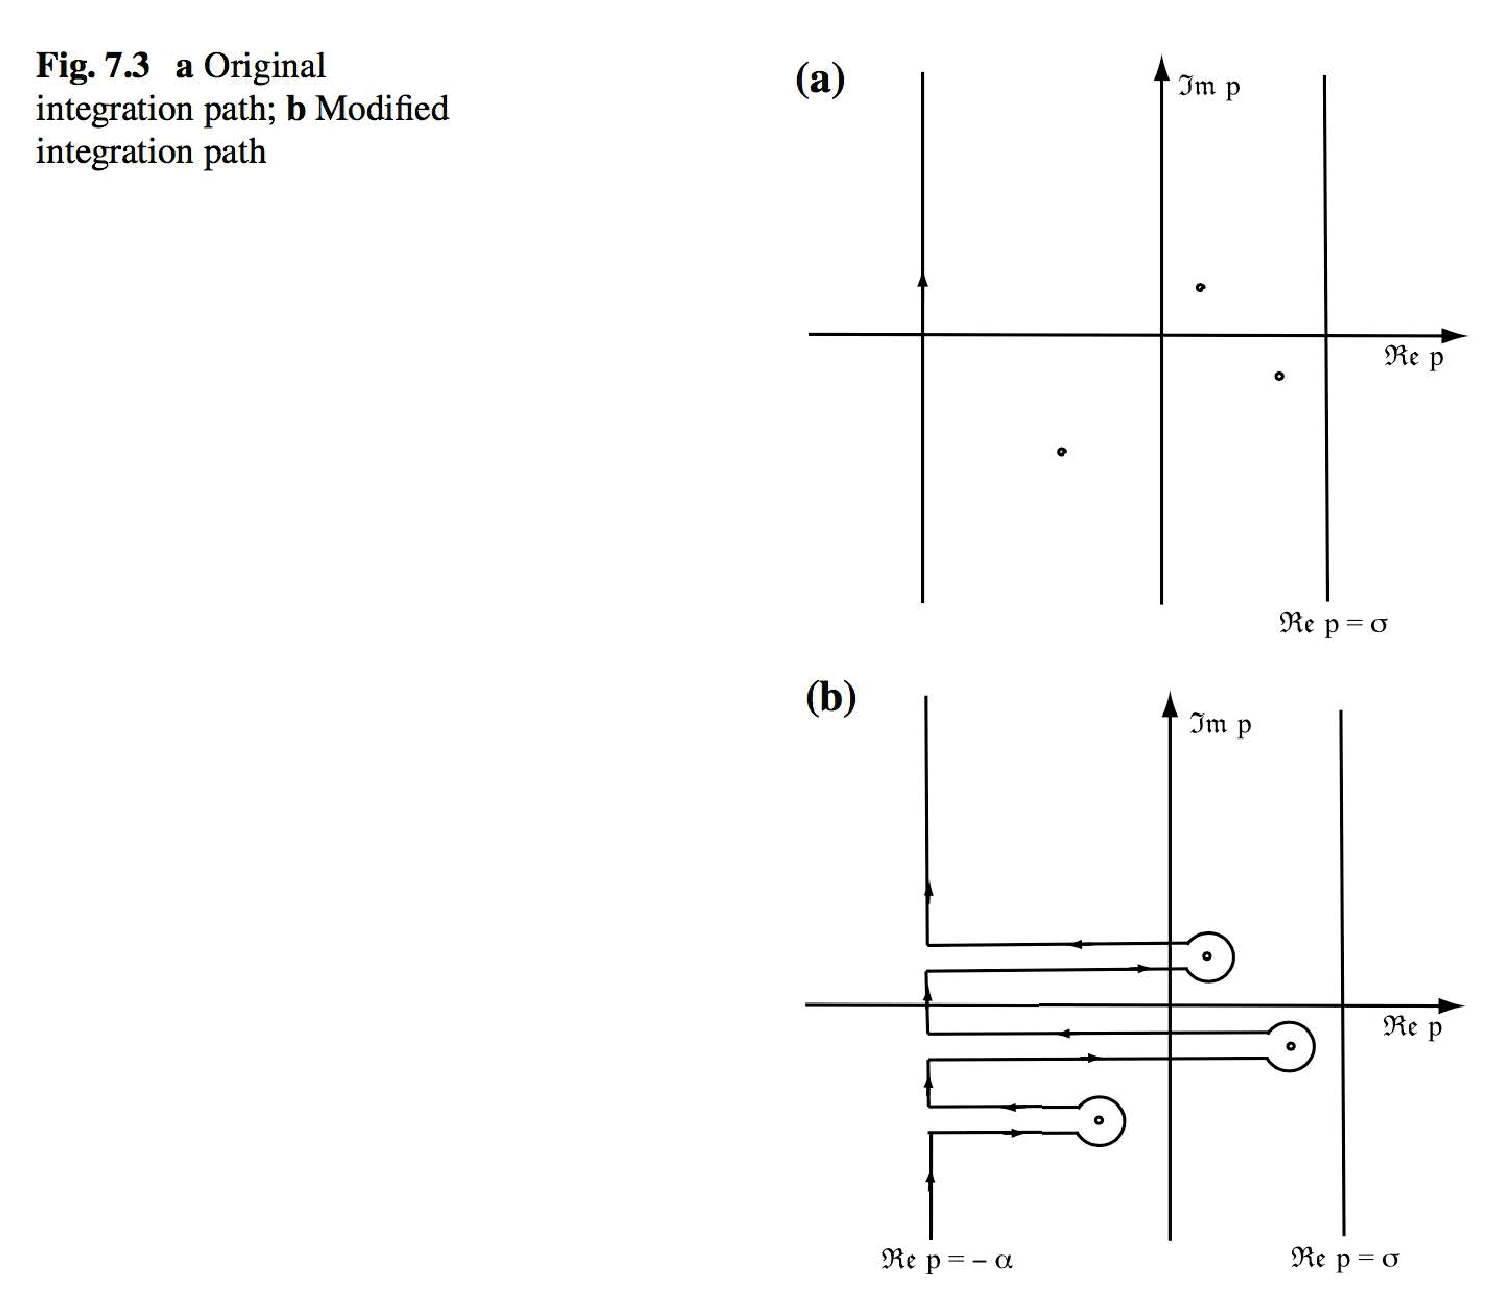
\includegraphics[height=10.cm, angle=0]{inlaplace.eps}
\caption{
a) Original integration path; b) Modified integration path.
}
\label{fig:inlaplace}
\end{figure*}
%===========================================================================================================================



The vertical segments of the integration path (where ${\rm Re}~ p = -\alpha$) do not contribute to the integral when $t \rightarrow +\infty$, because of the factor $e^{-\alpha t}$. The contributions from the oppositely directed horizontal segments cancel out as well. Thus the only part left is the contribution from the paths (of infinitesimal radius) circling the poles
\begin{align}
\tilde{E}(k, t) &= \frac{1}{2\pi i}  \oint \hat{E}(k, p) {\rm e}^{pt} \dif p ~.
\end{align}
If the solutions of the equation
\begin{equation}
D(k, p_j) = 0 ~,
\label{dispersion}
\end{equation}
are indicated by $p_j, (j = 1, 2, \cdots N)$, 
\begin{equation*}
\color{orange} p_j(k) = \gamma_j(k) -i\omega_j (k) ~,
\end{equation*}
and the expression for $\tilde{E}(k, t)$ is
\begin{equation}
\tilde{E}(k, t) = \sum_{j=1}^N R_j {\rm} e^{\gamma_j t} {\rm e}^{-i \omega_j t} ~,
\label{E_kt_residue}
\end{equation}
where \textcolor{blue}{$R_j$ is the residue of $\hat{E}(k, p)$ in $p = p_j$}. The electric field is given by a superposition of waves, whose amplitude increases or decreases exponentially with time, according to the sign of $\gamma$. All terms with $\gamma_j < 0$ represent \textcolor{green}{damped oscillations}, the more so the highest the value of $|\gamma_j|$. When the time elapsed from the initial excitation is sufficiently long, the dominant term will be the one corresponding to the \textcolor{blue}{pole closest to the imaginary axis of $p$}. The terms with $\gamma_j > 0$, on the other hand, represent \textcolor{green}{amplified oscillations} that very quickly get out of the linear regime. To stay within the framework of the present theory of small amplitude waves, we must assume that, even if poles with ${\rm Re}~ p > 0$ do exist, they lie close to the imaginary axis of $p$. In both cases, we are concerned only with poles of $D(k, p)$ whose $\gamma$ is sufficiently small, i.e. $|\gamma /\omega| \ll 1$.

For the dispersion relation of our low-amplitude electrostatic waves, i.e. Eq. (\ref{dispersion}), the integrand has a pole for \textcolor{yellow}{$u = \dfrac{ip}{k}$} in Eq. (\ref{D_kp}). The \textcolor{yellow}{Laplace transform had been defined for ${\rm Re}~ p > 0$, which implies that the pole lies in the half-space ${\rm Im}~ u > 0$, external to the integration path that runs along the real axis of $u$}. However, when deforming the integration path of the inverse Laplace transform, \textcolor{yellow}{it is assumed that ${\rm Re}~ p = \alpha < 0$}. We must \textcolor{yellow}{find an analytical continuation of the integral} entering Eq. (\ref{D_kp}) when ${\rm Re}~ p < 0$. Such a continuation is obtained, once again, by deforming the integration path so that the pole remains located above the new path, as shown in Fig. \ref{fig:landau}.

%===========================================================================================================================
\begin{figure*}
\centering
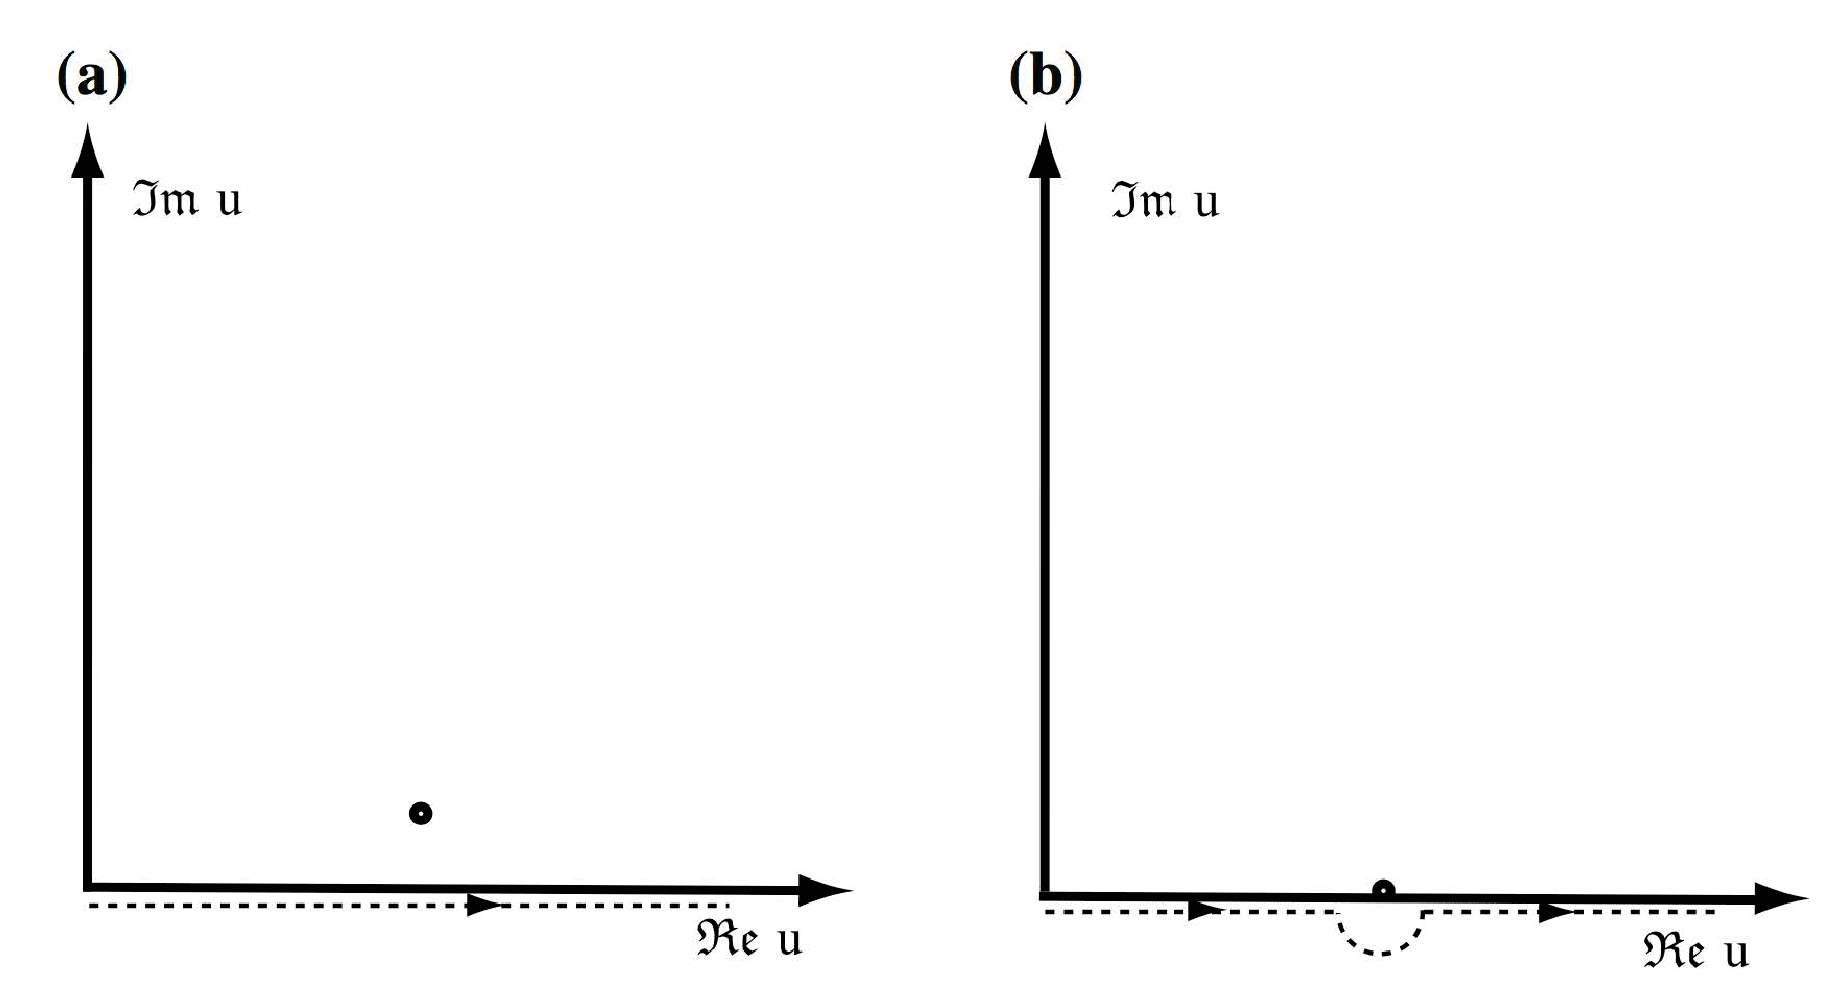
\includegraphics[height=8.cm, angle=0]{landau_prescrip.eps}
\caption{
The integration path according to the Landau prescription. a) Original path, b) Modified path.
}
\label{fig:landau}
\end{figure*}
%===========================================================================================================================

Making use of so-called \textcolor{red}{Landau prescription}, we can \textcolor{yellow}{define $D(k, p)$ for any value of $p$, in particular for ${\rm Re}~ p = \gamma  \rightarrow 0$}. The \textcolor{orange}{principal part of an integral in the complex plane} is defined as
\begin{equation*}
\color{orange} P \int\limits_{-\infty}^\infty \frac{f(z)}{z-z_0} \dif z = \underset{\epsilon\rightarrow 0}\lim \left[\int\limits_{-\infty}^{-\epsilon} \frac{f(z)}{z-z_0} \dif z +\int\limits_{\epsilon}^\infty \frac{f(z)}{z-z_0} \dif z \right] ~,
\end{equation*}
the integral appearing in Eq. (\ref{D_kp}) can be written as
\begin{align}
\nonumber \int_{-\infty}^\infty  \frac{1}{p+iku} \frac{\dif F_0}{\dif u}  \dif u &= \frac{1}{ik} \int_{-\infty}^\infty  \frac{F^\prime_0}{u-ip/k} \dif u \\
\nonumber &= \frac{1}{ik} \left[P \int_{-\infty}^\infty  \frac{F^\prime_0}{u-ip/k} \dif u +i\pi F^\prime_0\left(\dfrac{ip}{k} \right) \right] \\
&= P \int_{-\infty}^\infty  \frac{F^\prime_0}{p +iku} \dif u +\dfrac{\pi}{k} F^\prime_0\left(\dfrac{ip}{k} \right)
\end{align}
The dispersion relation will be given by the solution of the equation
\begin{align}
\nonumber D(k, p) &= 1 -i \frac{\omega^2_{pe} }{k} \left[ P \int_{-\infty}^\infty  \frac{F^\prime_0}{p +iku} \dif u +\dfrac{\pi}{k} F^\prime_0\left(\dfrac{ip}{k} \right) \right] \\
&= 1 +\omega^2_{pe} \left[ P \int_{-\infty}^\infty  \frac{F_0}{(p +iku)^2} \dif u -i\dfrac{\pi}{k^2} F^\prime_0\left(\dfrac{ip}{k} \right) \right] = 0 ~.
\end{align}
For small $k$-values, take a series expansion of $(p + iku)^{-2}$,
\begin{equation}
1 +\frac{\omega^2_{pe} }{p^2} \int_{-\infty}^\infty F_0\left(1- \frac{2iku}{p} -\frac{3k^2 u^2}{p^2} +\cdots \right) \dif u -i \frac{\pi \omega_{pe}^2}{k^2} F^\prime_0\left(\dfrac{ip}{k} \right) = 0 ~,
\end{equation}
where the imaginary terms in the integrand are odd functions of $u$ and therefore the corresponding integrals vanish, since $F_0$ is an even function. 
\begin{equation}
-p^2 \simeq \omega^2_{pe} \left(1 -\frac{3k^2 c_s^2}{p^2} \right) -i\frac{\pi \omega_{pe}^2}{k^2} F^\prime_0\left(\dfrac{ip}{k} \right) ~,
\label{disp_rela}
\end{equation}
where
\begin{align*}
\int_{-\infty}^\infty F_0 \dif u = 1 ~, ~~ \int_{-\infty}^\infty u^2 F_0 \dif u = \frac{k_B T}{m} = c_s^2 ~.
\end{align*}
In the limit \textcolor{red}{$k \rightarrow 0$}, the dispersion relation reduces to
\begin{equation*}
\textcolor{red}{?} -p^2 = \omega^2 -\gamma^2 +2i\gamma \omega = \omega^2_{pe} ~,
\end{equation*}
since $F_0$ and all its derivatives converge so fast when the argument tends to infinity that the last term of Eq. (\ref{disp_rela}) tends to zero. In this limit, $\gamma =0$ and the \textcolor{orange}{wave's electric field} given by Eq. (\ref{E_kt_residue}), \textcolor{orange}{is constant in time}. The wave frequency coincides with that of a Langmuir wave, $\omega = \pm \omega_{pe}$.

Waves whose \textcolor{yellow}{amplitude is time-dependent} appear when the corrections connected with \textcolor{red}{finite values of $k$} are taken into account. At the lowest order, keep the term in $k^2$ at the rhs of Eq. (\ref{disp_rela}), but replace $p^2$ with $-\omega^2_{pe}$, namely with the solution of zeroth-order in $k^2$. From the real part of Eq. (\ref{disp_rela}),
\begin{equation}
\color{red} \omega^2 = \omega^2_{pe} +3k^2 c_s^2 ~, 
\end{equation}
which is the \textcolor{orange}{dispersion relation of Langmuir waves corrected for thermal effects}. The imaginary part of Eq. (\ref{disp_rela}) gives 
\begin{equation}
\gamma = \frac{\pi}{2} \frac{\omega_{pe}^3}{k^2} F^\prime_0\left(\dfrac{\omega_{pe}}{k} \right)
\end{equation}
The sign of $\gamma$ depends upon the sign of the first derivative of the equilibrium distribution function, taken at the position where the speed of the particles equals the phase velocity of the wave. The damping is thus related to the resonant interaction of a particular group of particles with the electrostatic wave. This phenomenon does not show up in a fluid description, where the ``anomalous" behaviour of a group of peculiar particles is cancelled by the process of averaging over the velocities that lies at the basis of those models. Since the (maxwellian) equilibrium function is a decreasing function of the velocity for $u > 0$, $\gamma$ will have negative values and the wave will be subject to the so-called \textcolor{red}{Landau damping}.



\begin{equation}
\gamma = -\frac{\pi}{2} \frac{\omega_{pe}^3}{k^2} F^\prime_0\left(-\dfrac{\omega_{pe}}{|k|} \right) ~,
\end{equation}


\begin{equation}
\gamma = -\frac{\pi}{8} \frac{\omega_{pe}}{|k \lambda_D|^3} \exp\left[-\dfrac{1}{2(k\lambda_D)^2} -\dfrac{3}{2} \right] ~,
\end{equation}

\begin{equation*}
\omega_{pe} \lambda_D = c_s ~,
\end{equation*}


The equation of motion of the test electron, with energy slightly higher than the minimum of $V$, is
\begin{equation*}
m\ddot{x} = -eE = -eE_0 \sin(kx) \simeq -eE_0 k x ~,
\end{equation*}
from which it follows that the particles trapped close to the region of minimum potential energy will harmonically oscillate with a frequency
\begin{equation*}
\omega_b = \sqrt{\dfrac{eE_0 k}{m_e} } = k \sqrt{\dfrac{e\phi_0}{m_e} }
\end{equation*}

\begin{equation*}
\dfrac{\tau_b}{\tau_{pe}} \simeq \frac{\omega_{pe}}{k c_s} \sqrt{\frac{k_B T}{e \Phi_0} } \gg 1 ~,
\end{equation*}



The linear phase of the Landau damping might last for many wave periods.

\cite{Plasma2014} We shall investigate \textcolor{red}{electromagnetic wave propagation through a warm collisionless plasma}, extending to take \textcolor{red}{thermal effects} into account. It turns out that the \textcolor{red}{thermal modifications to wave propagation are not particularly well described by fluid equations}.

 the \textcolor{blue}{propagation of small amplitude plasma waves through a uniform plasma} possessing \textcolor{blue}{no equilibrium magnetic field}. We shall \textcolor{blue}{only consider electron motion}, assuming that the \textcolor{blue}{ions form an immobile, neutralizing background}. The \textcolor{blue}{ions are also assumed to be singly charged}. We shall search for \textcolor{red}{electrostatic plasma waves}. Such waves are \textcolor{red}{longitudinal} in nature (i.e., $\vec{E} \propto \vec{k}$), and possess a \textcolor{red}{perturbed electric field}, but \textcolor{red}{no perturbed magnetic field}.

The Vlasov equation for an unmagnetized, collisionless plasma is
\begin{equation*}
\dfrac{\partial f_e}{\partial t} + \vec{v}\cdot \nabla f_e - \dfrac{e}{m_e} \vec{E} \cdot \nabla_v f_e = 0 ~,
\end{equation*}
where $f_e(\vec{r}, \vec{v}, t)$ is the ensemble-averaged electron distribution function. The electric field satisfies
\begin{equation}
\vec{E} = -\nabla \phi ~,
\end{equation}
where
\begin{equation}
\nabla^2 \phi = -\dfrac{e}{\epsilon_0} \left(n -\int f_e \dif^3 \vec{v} \right) ~.
\end{equation}
$n$ is the number density of ions (which is the same as the equilibrium number density of electrons). For the small amplitude waves, it is appropriate to linearize the Vlasov equation. Suppose that the electron distribution function is written
\begin{equation}
f_e(\vec{r}, \vec{v}, t) = f_0(\vec{r}, \vec{v}, t) +f_1(\vec{r}, \vec{v}, t) ~.
\end{equation}
$f_0$ represents the equilibrium electron distribution, whereas $f_1$ represents the small perturbation due to the wave. $\int f_0 \dif^3 \vec{v} = n$. The electric field is assumed to be zero in the unperturbed state, $\vec{E}(\vec{r}, t)$ can be regarded as a small quantity.
\begin{align}
& \dfrac{\partial f_1}{\partial t} + \vec{v}\cdot \nabla f_1 - \dfrac{e}{m_e} \vec{E} \cdot \nabla_v f_0 = 0 ~, \\
& \nabla^2 \phi = \dfrac{e}{\epsilon_0} \int f_1 \dif^3 \vec{v} ~.
\end{align}

\begin{align}
& -i(\omega -\vec{k}\cdot \vec{v}) f_1 + i\dfrac{e}{m_e} \phi \vec{k}\cdot \nabla_v f_0 = 0 ~, \\
& -k^2 \phi = \dfrac{e}{\epsilon_0} \int f_1 \dif^3 \vec{v} ~,
\end{align}


If $\phi$ is non-zero then we must have
\begin{equation}
1 + \dfrac{e^2}{\epsilon_0 m_e k^2} \int \dfrac{\vec{k}\cdot \nabla_v f_0}{\omega -\vec{k}\cdot \vec{v}} \dif^3 \vec{v} = 0 ~.
\label{eq:dispersion}
\end{equation}
We can interpret Equ. (\ref{eq:dispersion}) as the dispersion relation for electrostatic plasma waves, relating the wavevector, $\vec{k}$, to the frequency, $\omega$. However, in doing so, we run up against a serious problem, because the \textcolor{red}{integral has a singularity in velocity space}, where \textcolor{red}{$\omega = \vec{k}\cdot \vec{v}$}, and is, therefore, \textcolor{red}{not properly defined}. Landau showed that, instead of simply assuming that $f_1$ varies in time as $\exp(-i \omega t)$, the problem must be regarded as an ``initial value problem" in which $f_1$ is specified at $t = 0$, and calculated at later times. 
\begin{equation}
f_1(\vec{r}, \vec{v}, t) = f_1(\vec{v}, t) \exp (i\vec{k}\cdot \vec{r}) ~.
\end{equation}
Define $u$ as the velocity component along $\vec{k}$ (i.e., $u = \vec{k} \cdot \vec{v}/k$), and to also define $F_0(u)$ and $F_1(u, t)$ as the integrals of $f_0(\vec{v})$ and $f_1(\vec{v}, t)$, respectively, over the velocity components perpendicular to $\vec{k}$.
\begin{align}
& \dfrac{\partial F_1}{\partial t} +iku F_1 - \dfrac{e}{m_e} E \dfrac{\partial F_0}{\partial u}  = 0 ~, \\
& ik E = -\dfrac{e}{\epsilon_0} \int_{-\infty}^\infty F_1(u) \dif u ~,
\end{align}
where $\vec{E} = E\vec{k}/k$.
\begin{equation}
\overline{F}_1(u,p) = \int_0^\infty F_1(u,t) {\rm e}^{-pt} \dif t ~.
\end{equation}
If the rate of increase of $F_1$ with increasing $t$ is no faster than exponential, then the integral on the right-hand side of the previous equation converges, and defines $\overline{F}_1$ as an analytic function of $p$, provided that the real part of $p$ is sufficiently large.
\begin{align}
& p\overline{F}_1 +iku \overline{F}_1 = \dfrac{e}{m_e} \overline{E} \dfrac{\partial F_0}{\partial u} + F_1(u, t=0) ~, \\
& ik\overline{E} = -\dfrac{e}{\epsilon_0} \int_{-\infty}^\infty \overline{F}_1(u) \dif u ~.
\end{align}

\begin{align}
& ik\overline{E} = -\dfrac{e}{\epsilon_0} \int_{-\infty}^\infty \left[\dfrac{e}{m_e} \overline{E} \dfrac{\partial F_0/\partial u}{p+iku} +\dfrac{F_1(u,t=0)}{p+iku} \right] \dif u ~, \\
& \overline{E}(p) = -\dfrac{e/\epsilon_0}{ik\epsilon(k,p)} \int_{-\infty}^\infty \dfrac{F_1(u,t=0)}{p+iku}  \dif u
\end{align}
where
\begin{equation}
\epsilon(k,p) = 1+ \dfrac{e^2}{\epsilon_0 m_e k} \int_{-\infty}^\infty \dfrac{\partial F_0/\partial u}{ip -ku} \dif u ~.
\end{equation}
$\epsilon(k,p)$ is known as the \textcolor{red}{plasma dielectric function}. If $p$ is replaced by $-i \omega$, the dielectric function becomes equivalent to the left-hand side of Equ. (\ref{eq:dispersion}). However, because p possesses a positive real part, the integral on the right-hand side of the previous equation is well defined. The Laplace transform of the distribution function is written
\begin{equation}
\overline{F}_1 = \dfrac{e}{m_e} \overline{E} \dfrac{\partial F_0/\partial u}{p +iku} + \dfrac{F_1(u,t=0)}{p+iku} ~,
\end{equation}
or 
\begin{equation}
\overline{F}_1(u,p) = -\dfrac{e^2}{\epsilon_0 m_e ik} \dfrac{\partial F_0/\partial u}{\epsilon(k,p)(p +iku)} \int_{-\infty}^\infty  \dfrac{F_1(u^\prime,t=0)}{p+iku^\prime} \dif u^\prime + \dfrac{F_1(u,t=0)}{p+iku} ~.
\end{equation}

The inverse Laplace transform of the distribution function is given by
\begin{equation}
F_1(u,t) = \dfrac{1}{2\pi i} \int_C \overline{F}_1 (u,p) e^{pt} \dif p ~,
\end{equation}
where $C$ - the so-called \textcolor{red}{Bromwich contour} - is \textcolor{orange}{a contour running parallel to the imaginary axis, and lying to the right of all singularities (otherwise known as poles) of $\overline{F}_1$} in the complex-$p$ plane, see Fig. \ref{fig:Bromwich_c}. There is an analogous expression for the parallel electric field, $E(t)$.

%===========================================================================================================================
\begin{figure*}
\centering
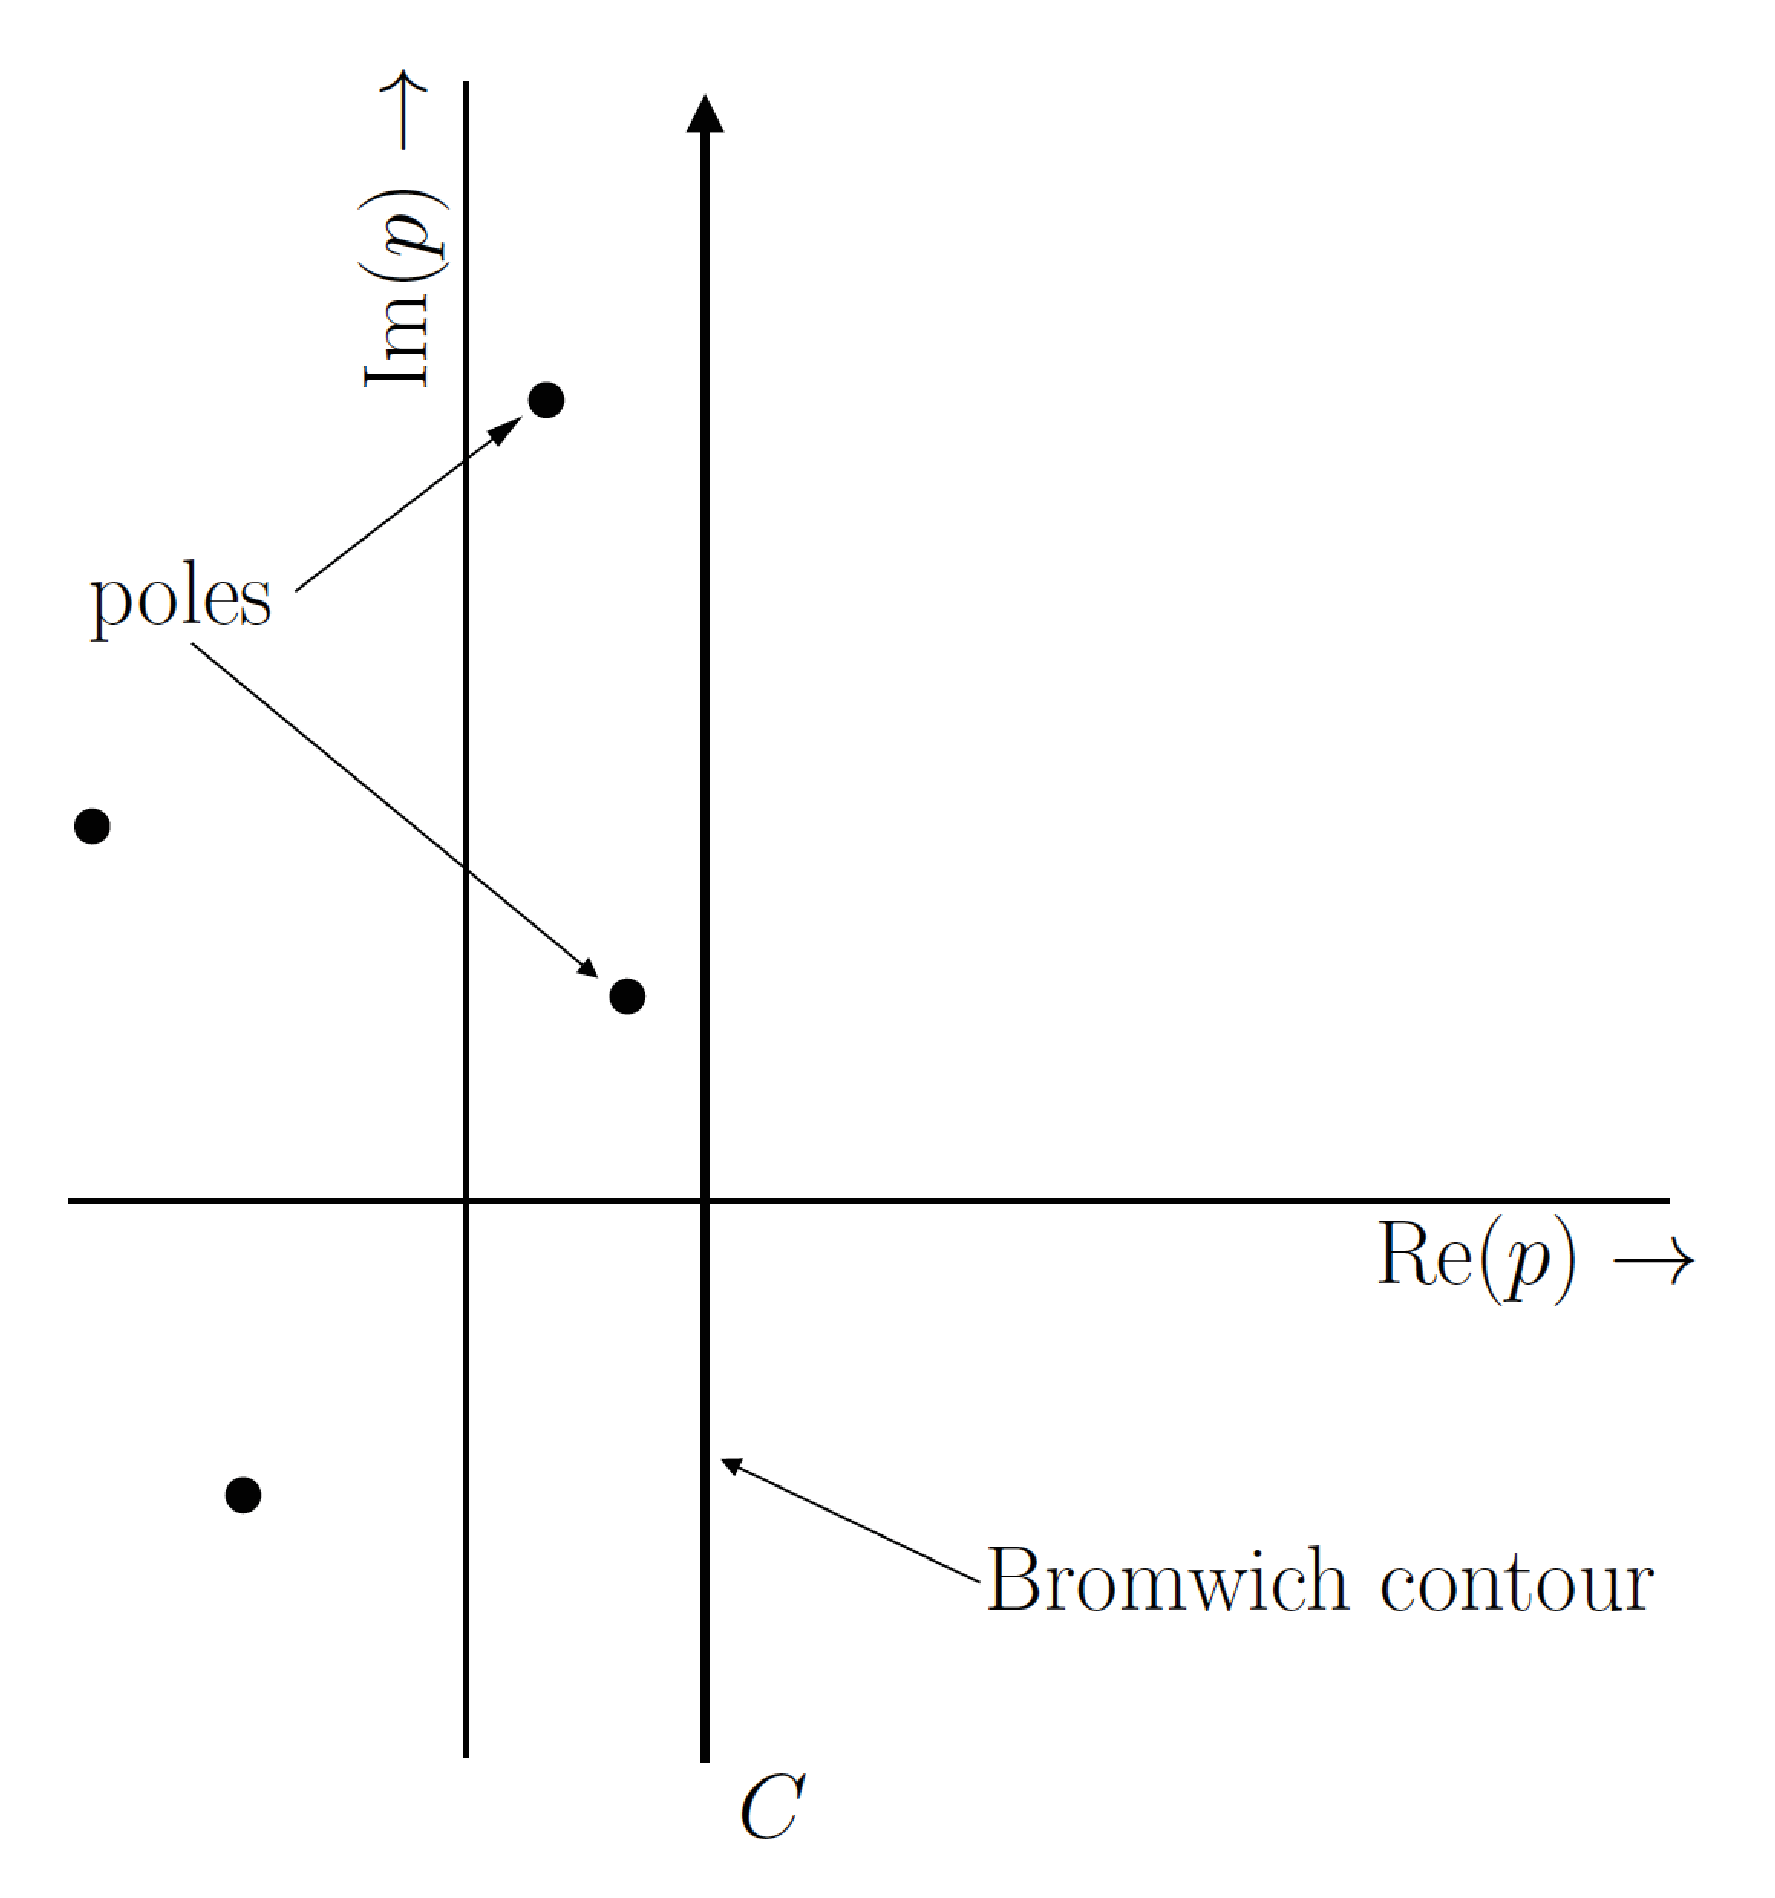
\includegraphics[height=8.cm, angle=0]{Bromwich_contour.eps}
\caption{
The Bromwich contour.
}
\label{fig:Bromwich_c}
\end{figure*}
%===========================================================================================================================

Rather than trying to obtain a general expression for $F_1(u,t)$, we shall concentrate on the behavior of the perturbed distribution function at large times. If $\overline{F}_1(u, p)$ has only a finite number of simple poles in the region ${\rm Re}(p) > -\sigma$ (where $\sigma$ is real and positive) then we may deform the contour as shown in Fig. \ref{fig:dBromwich_c}, with a loop around each of the singularities. A pole at $p_0$ gives a contribution that varies in time as $e^{p_0 t}$, whereas the vertical part of the contour gives a contribution that varies as $e^{-\sigma t}$. For sufficiently large times, the latter contribution is negligible, and the behavior is dominated by contributions from the poles furthest to the right. 
 
 
%===========================================================================================================================
\begin{figure*}
\centering
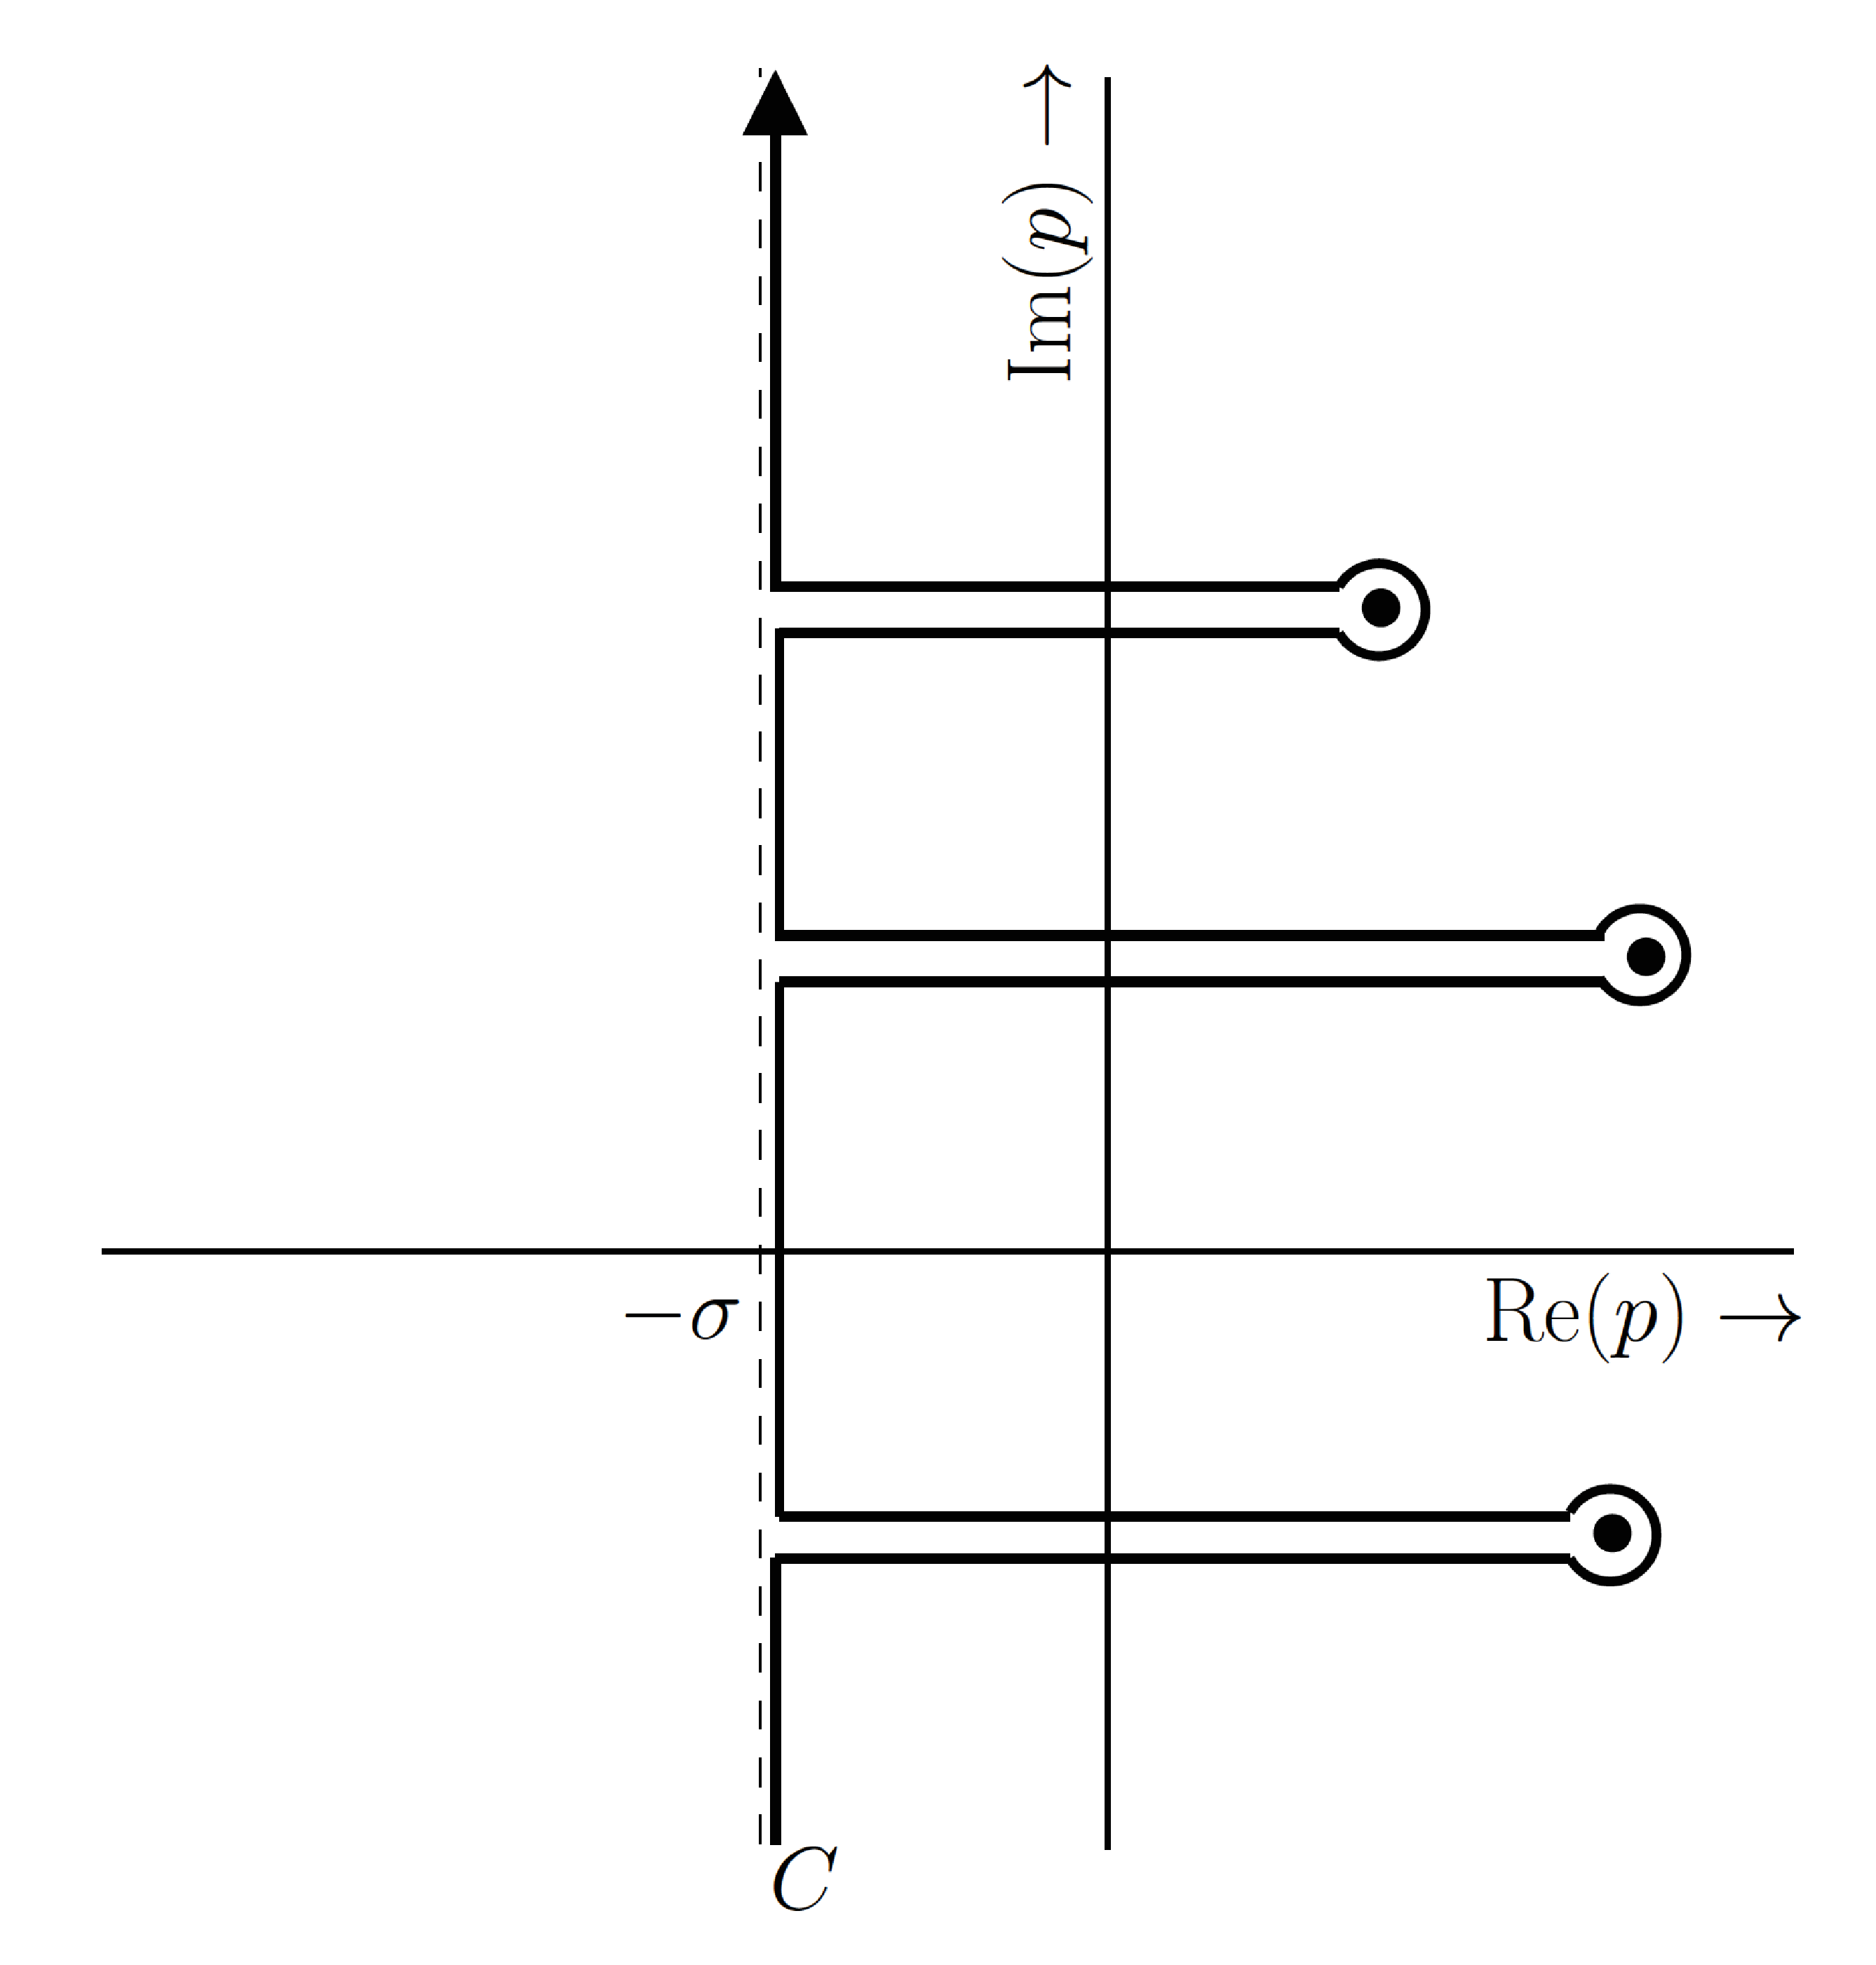
\includegraphics[height=8.cm, angle=0]{distorted_Bromwich_contour.eps}
\caption{
The distorted Bromwich contour.
}
\label{fig:dBromwich_c}
\end{figure*}
%===========================================================================================================================
 
\begin{equation}
\int_{-\infty}^\infty \dfrac{G(u)}{u-ip/k} \dif u ~.
\label{eq:integral}
\end{equation}
Such integrals become singular as $p$ approaches the imaginary axis. In order to distort the contour $C$ as shown in Fig. \ref{fig:dBromwich_c}, we need to continue these integrals smoothly across the imaginary $p$-axis. As a consequence of the way in which the Laplace transform was originally defined - that is, for ${\rm Re}(p)$ sufficiently large - the appropriate way to do this is to take the values of these integrals when $p$ lies in the right-hand half-plane, and to then find the analytic continuation into the left-hand half-plane. 
 
If $G(u)$ is sufficiently well-behaved that it can be continued off the real axis as an analytic function of a complex variable $u$, then the continuation of (\ref{eq:integral}) as the singularity crosses the real axis in the complex $u$-plane, from the upper to the lower half-plane, is obtained by letting the singularity take the contour with it.
 
Note that the ability to deform the Bromwich contour into that of Fig. \ref{fig:Bromwich_cLandau}, and so to find a dominant contribution to $E(t)$ and $F_1(u, t)$ from a few poles, depends on $F_0(u)$ and $F_1(u,t = 0)$ having smooth enough velocity dependences that the integrals appearing in Equations (8.17), (8.18), and (8.20) can be analytically continued sufficiently far into the lower half of the complex $u$-plane. 

%===========================================================================================================================
\begin{figure*}
\centering
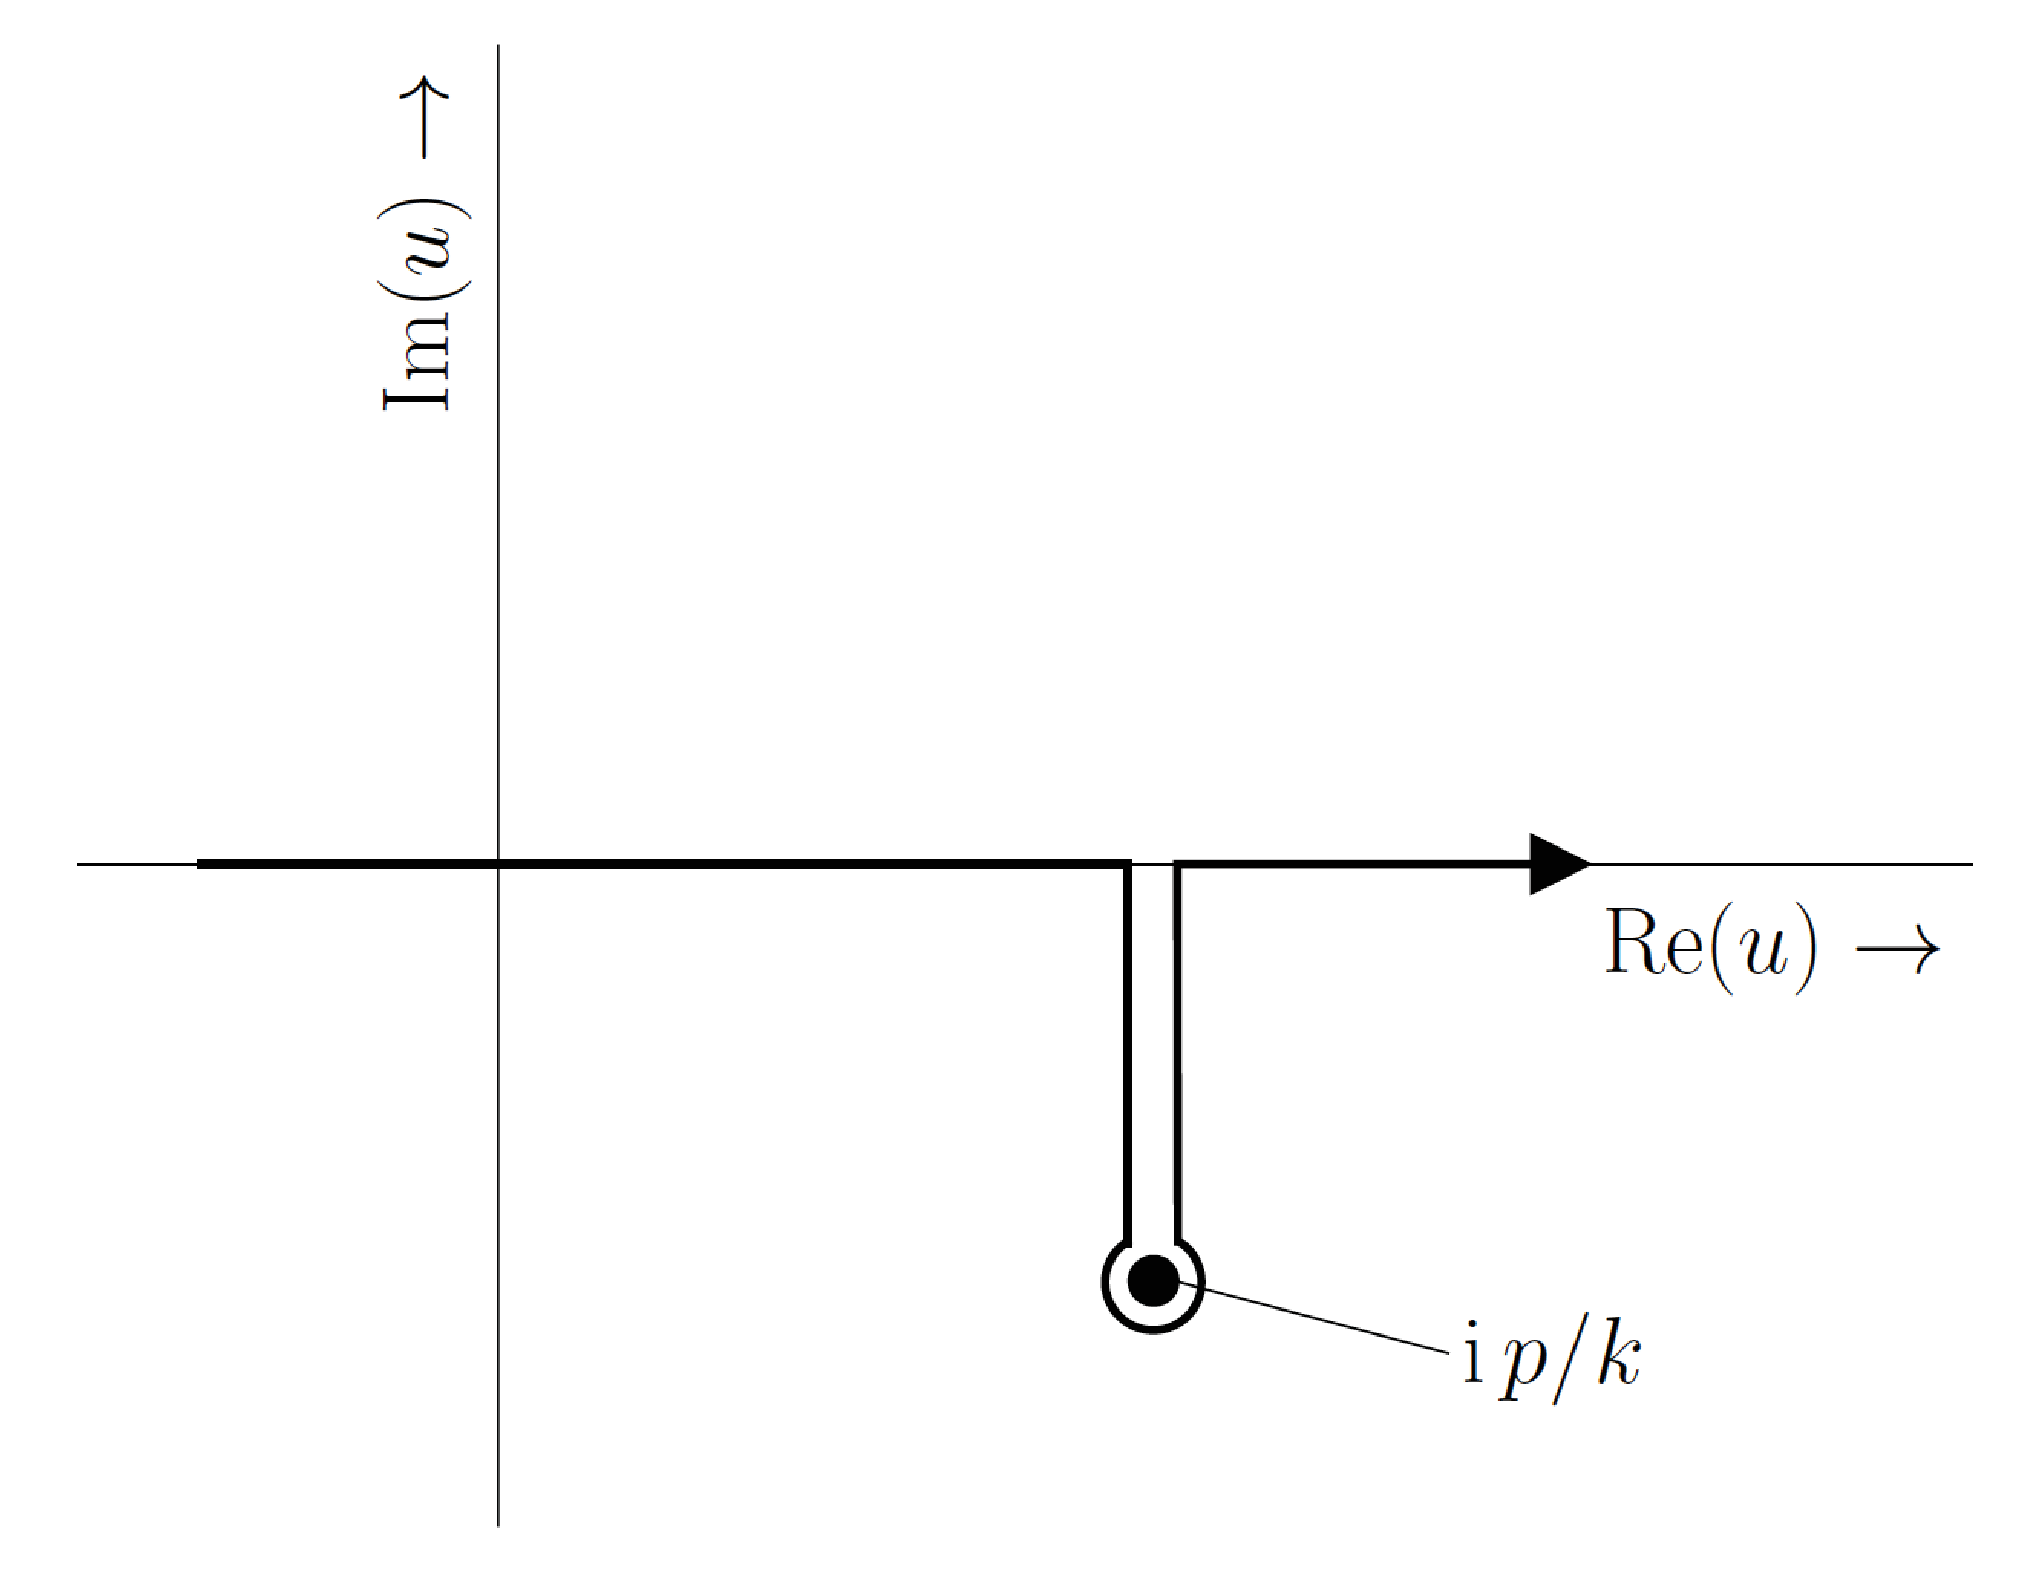
\includegraphics[height=8.cm, angle=0]{Bromwich_contour_for_Landau_damping.eps}
\caption{
The Bromwich contour for Landau damping.
}
\label{fig:Bromwich_cLandau}
\end{figure*}
%===========================================================================================================================

If we consider the electric field given by the inversion of Equation (8.17), then we see that its behavior at large times is dominated by the zero of $\epsilon(k, p)$ that lies furthest to the right in the complex $p$-plane. According to Equations (8.20) and (8.21), F1(u, t) has a similar contribution, as well as a contribution that varies in time as e−i k u t . Thus, for sufficiently long times after the initial excitation of the wave, the electric field depends only on the positions of the roots of ε(k, p) = 0 in the complex p-plane. The distribution function, on the other hand, has corresponding components from these roots, as well as a component that varies in time as e−i k u t . At large times, the latter component of the distribution function is a rapidly oscillating function of velocity, and its contribution to the charge density, obtained by integrating over u, is negligible.
 
As we have already noted, the function ε(k, p) is equivalent to the left-hand side of Equation (8.9), provided that p is replaced by −i ω. Thus, the dispersion relation, (8.9), obtained via Fourier transformation of the Vlasov equation, gives the correct behavior at large times, as long as the singular integral is treated correctly. Adapting the procedure that we discovered using the complex variable p, we see that the inte- gral is defined as it is written for Im(ω) > 0, and analytically continued, by deform- ing the contour of integration in the u-plane (as shown in Figure 8.3), into the region Im(ω) < 0. The simplest way to remember how to do the analytic continuation is to observe that the integral is continued from the part of the ω-plane corresponding to growing perturbations to that corresponding to damped perturbations. Once we know this rule, we can obtain kinetic dispersion relations in a fairly direct manner, via Fourier transformation of the Vlasov equation, and there is no need to attempt the more complicated Laplace transform solution.
 
%%%%%%%%%%%%%%%%%%%%%%%%%%%%%%%%%%%%%%%%%%%%%%%%%%%%%%%%%%%%%%%%%%%%%%
\bibliographystyle{unsrt_update}
\bibliography{ref}
%%%%%%%%%%%%%%%%%%%%%%%%%%%%%%%%%%%%%%%%%%%%%%%%%%%%%%%%%%%%%%%%%%%%%%

\end{document}